\documentclass[a4paper,11pt]{kth-mag}

\usepackage{silence}
\WarningFilter{glossaries}{Overriding \printglossary}
\WarningFilter{glossaries}{Overriding `theglossary'}

\usepackage[T1]{fontenc}
\usepackage{textcomp}
\usepackage{lmodern}
\usepackage[utf8]{inputenc}
\usepackage{csquotes}
\usepackage[swedish,english]{babel}
\usepackage{modifications}
\usepackage[backend=biber]{biblatex}
\usepackage{hyperref}
\hypersetup{
}
\usepackage{listings}
\usepackage{tikz}
\usetikzlibrary{arrows,positioning,fit,calc,decorations.markings}
\usepackage{todonotes}
\usepackage[toc,acronym]{glossaries}
\makenoidxglossaries
% \makeglossaries

\lstset{%
  frame=L,
  basicstyle=\tiny,
  xleftmargin=\parindent
}

\bibliography{bibliography.bib}

\newcommand{\code}[1]{\texttt{#1}}
\newcommand\abbr[2][]{\uppercase{#2}\ifthenelse{\equal{#1}{}}%
                     {}{#1}}

\newenvironment{metatext}{%
  \textbf{$\hookrightarrow$}
  \begin{itshape}
}{
  \end{itshape}
  \newline
  \newline
  \useignorespacesandallpars
}

\def\useignorespacesandallpars#1\ignorespaces\fi{%
#1\fi\ignorespacesandallpars}


\makeatletter
\def\ignorespacesandallpars{%
  \@ifnextchar\par
    {\expandafter\ignorespacesandallpars\@gobble}%
    {}%
}
\makeatother

\newglossaryentry{self-contained}{
  name=self-contained,
  description={A self-contained module handles its task without any help from the user of the module}
}
\newglossaryentry{web} {
  name=web,
  description={Short for the world wide web}
}
\newglossaryentry{gls-wysiwyg}{
  name=WYSIWYG,
  description={A classification that ensures that text and graphics during editing appears close to the result}
}
\newglossaryentry{fork}{
  name=fork,
  description={When developers copy the source code of a project to start independent development on it creating a separate piece of software. The new code is often rebranded to avoid confusion. Common in the open source community}
}
\newglossaryentry{WebKit}{
  name=WebKit,
  description={The open source \gls{layout engine} used by Safari. Google's Blink \gls{layout engine} is a recent \gls{fork} of WebKit}
}
\newglossaryentry{HTML5}{
  name=HTML5,
  description={The fifth revision of the \gls{HTML} standard}
}
\newglossaryentry{CSS3}{
  name=CSS3,
  description={The third revision of the \gls{CSS} standard}
}
\newglossaryentry{responsive}{
  name=responsive,
  description={Elements and content of the \gls{document} can detect size changes and act accordingly. Usually a restructure of content is performed at certain breakpoints}
}
\newglossaryentry{render tree}{
  name={render tree},
  description={Used by \glspl{layout engine} as the model for the visual representation of the document}
}
\newglossaryentry{media queries}{
  name={media queries},
  description={The CSS feature of specifying conditional style rules for elements by conditions such as the viewport size}
}
\newglossaryentry{viewport}{
  name={viewport},
  description={The outer frame that defines the visible area of the \gls{document}. Usually defined by the \gls{browser} window, but may be restricted by other factors such as frames}
}
\newglossaryentry{element}{
  name={element},
  description={HTML \glspl{document} consists of elements, which can be regarded as the building blocks of \gls{web} pages. A \gls{web} page describes a tree structure of elements and text}
}
\newglossaryentry{native}{
  name={native},
  description={Refers to \glspl{API} and systems implemented and provided by \glspl{browser}. Such \glspl{API} and systems are often described by standards specifications}
}
\newglossaryentry{third-party}{
  name={third-party},
  description={Refers to \glspl{API} and systems implemented on top of the \gls{browser}, usually in \gls{JavaScript}. Such \glspl{API} and systems must be included by developers into the \gls{document}, and are usually not described by standards specifications}
}
\newglossaryentry{hypertext}{
  name={hypertext},
  description={\Glspl{document} with text and media with links (hyperlinks) to other \glspl{document} immediately accessible for the user. Often used as a synonym for hypermedia}
}
\newglossaryentry{JavaScript}{
  name={JavaScript},
  description={\Gls{native} \gls{browser} script language. \Gls{web} \glspl{document} often include JavaScript to make the \glspl{document} more dynamic and interactable}
}
\newglossaryentry{browser}{
  name={browser},
  description={Client application for navigating the \gls{WWW} and displaying \gls{web} pages. More formally known as a user agent}
}
\newglossaryentry{Java applet}{
  name={Java applet},
  description={A Java applet is a small application which is written in Java and delivered to users in the form of bytecode. See \url{www.java.com}}
}
\newglossaryentry{Flash}{
  name={Flash},
  description={Flash is a multimedia and software platform for producing cross platform interactive animations. See \url{www.flash.com}}
}
\newglossaryentry{StatCounter}{
  name={StatCounter},
  description={Collects and aggregates on a sample exceeding 15 billion page views per month collected from across the StatCounter network of more than 3 million websites}
}
\newglossaryentry{layout engine}{
  name={layout engine},
  description={The part of the browser that handles parsing, laying out and rendering \gls{web} content. Layout engines are often open source and browsers usually acts as a shell on top of a layout engine. Sometimes also called rendering engines}
}
\newglossaryentry{document}{
  name={document},
  description={Strictly defined as something that has a \gls{URI} and can return representations of the identified resource in response to \gls{HTTP} requests. If otherwise states, document will refer to \gls{HTML} \gls{web} pages in this thesis. In \gls{JavaScript}, document refers to the \gls{DOM} root}
}
\newglossaryentry{XHTML}{
  name={XHTML},
  description={Well-formed \gls{XML}-based markup language that extends or mirros \gls{HTML}. May be parsed by \gls{XML} parsers since it conforms to the stricter \gls{XML} syntax}
}

\newacronym{W3C}{W3C}{World Wide Web Consortium}
\newacronym{CSS}{CSS}{Cascading Style Sheets}
\newacronym{HTML}{HTML}{HyperText Markup Language}
\newacronym{DHTML}{DHTML}{Dynamic \gls{HTML}}
\newacronym{API}{API}{Application Program Interface}
\newacronym{RICG}{RICG}{Responsive Issues Community Group}
\newacronym{TCP}{TCP}{Transmission Control Protocol}
\newacronym{IP}{IP}{Internet Protocol}
\newacronym{ARPANET}{ARPANET}{Advanced Research Projects Agency Network}
\newacronym{ICANN}{ICANN}{Internet Corporation for Assigned Names and Numbers}
\newacronym{ISP}{ISP}{Internet Service Provider}
\newacronym{WWW}{WWW}{World Wide Web}
\newacronym{HTTP}{HTTP}{HyperText Transfer Protocol}
\newacronym{ICCC}{ICCC}{International Computer Communication Conference}
\newacronym{FTP}{FTP}{File Transfer Protocol}
\newacronym{US}{US}{United States}
\newacronym{DOD}{DOD}{Department Of Defense}
\newacronym{MILNET}{MILNET}{Military Network}
\newacronym{CSNET}{CSNET}{Computer Science Network}
\newacronym{NSF}{NSF}{National Science Foundation}
\newacronym{NSFNET}{NSFNET}{National Science Foundation Network}
\newacronym[see={[Glossary:]{gls-wysiwyg}}]{WYSIWYG}{WYSIWYG}{What You See Is What You Get\glsadd{gls-wysiwyg}}
\newacronym{GUI}{GUI}{Graphical User Interface}
\newacronym{NCSA}{NCSA}{National Center for Supercomputing Applications}
\newacronym{KDE}{KDE}{K Desktop Environment}
\newacronym{CGI}{CGI}{Common Gateway Interface}
\newacronym{XML}{XML}{EXtensible Markup Language}
\newacronym{AJAX}{AJAX}{Asynchronous \gls{JavaScript} and \acrshort{XML}}
\newacronym{WHATWG}{WHATWG}{Web Hypertext Application Technology Working Group}
\newacronym{RWD}{RWD}{Responsive Web Design}
\newacronym{DOM}{DOM}{Document Object Model}
\newacronym{URI}{URI}{Unique Resource Identifier}
\newacronym{CPU}{CPU}{Central Processing Unit}
\newacronym{DARPA}{DARPA}{Defense Advanced Research Projects Agency}
\newacronym{CERN}{CERN}{Conseil Europeen pour la Recherche Nucleaire}
\newacronym{OS}{OS}{Operating System}


\title{Modular responsive web design}
\foreigntitle{Modulär responsiv webbutveckling}
\subtitle{Allowing responsive web modules to respond to custom criteria instead of only the viewport size by implementing \emph{element queries}}
\author{Lucas Wiener \\ \lowercase{lwiener@kth.se}}
\date{February 2015}
\blurb{Master's Thesis at \abbr{csc}\\\hfill\\ Supervisors at \abbr{evry ab}: Tomas Ekholm \& Stefan Sennerö\\Supervisor at \abbr{csc}: Philipp Haller\\Examiner: Mads Dam}
\trita{TRITA xxx yyyy-nn}
\begin{document}
  \frontmatter
  \pagestyle{empty}
  \removepagenumbers
  \maketitle
  \selectlanguage{english}
  \begin{abstract}
    Abstract goes here.
  \end{abstract}
  \clearpage
  \begin{foreignabstract}{swedish}
    Sammanfattning ska vara här.
  \end{foreignabstract}
  \clearpage
  \tableofcontents*
  \listoftodos
  \mainmatter
  \pagestyle{newchap}
  \chapter{Introduction}
    \todo[inline]{Container or parent element? Using both now.}
    \todo[inline]{Rename framework to library?}
    \todo[inline]{Write about the targeted browser compatibility. Started writing about this but put it on hold in the appendix.}
    \todo[inline]{Word says that all "their own" is wrong.}
    \todo[inline]{Change all wikipedia sources to the real sources}
    \todo[inline]{Change self-contained to encapsulated?}
    \section{Targeted audience}
      This thesis is targeted for \gls{web} developers that wish to gain a deeper understanding of element queries and how one could solve the problem today.
      Heavy use of \gls{web} terminology is being used and intermediate \gls{web} development knowledge is assumed.
      \todo[inline]{Philipp wanted this to be more general.}
    \section{Problem statement}
      By using \gls{CSS} \gls{media queries}, developers can specify different style rules for different \gls{viewport} sizes.
      This is fundamental to creating \gls{responsive} \gls{web} applications.
      If developers want to build modular applications by composing the application by smaller components (\glspl{element}, scripts, styles, etc.) \gls{media queries} are no longer applicable.
      Modular \gls{responsive} components should be able to react and change style depending on the size that the component has been given by the application, not the \gls{viewport} size.
      The problem can be formulated as: \emph{It is not possible to specify conditional style rules for \glspl{element} depending on the size of an element}.
      See the included document in section~\ref{sec:problem-formulation} of the appendix for a more practical problem formulation.

      \todo{Is W3C okay with this? No they are not. Need to reformulate.}
      The main international standards organization for the \gls{web}, the \gls{W3C}, has unofficially stated that such feature would be infeasible to implement.
      Participants of the \gls{W3C}, which include both paying members and the public, are interested in solving the problem and possible solutions are being discussed.
      However, they are still at the initial planning stage so a solution will not be implemented \glslink{native}{natively} in the near future.
      While awaiting a \gls{native} solution it is up to the developers to implement this feature as a \gls{third-party} solution.
      Efforts have been made to create a robust \gls{third-party} solution, with moderate success.
      Since all current \gls{third-party} solutions have shortcomings, there is still no de facto solution that developers use and the problem remains unsolved.
      Some problems with implementing element queries \glslink{native}{natively} in \gls{CSS} are:
      \begin{itemize}
        \item \textbf{Circularity:}
        If style rules can be applied by criteria of other \glspl{element}, it is possible to create cyclic rules (infinite loops of styling).
        Some cyclic rules might be possible to detect during \gls{CSS} parsing, but there are so many combinations of style properties that could result in cyclic rules that it will add a lot of complexity to the language, both for implementers and users.
        Also, it has been shown that some cyclic rules are impossible to detect at parsetime, due to being dependent on runtime factors.
        \item \textbf{Performance:} 
        \Gls{layout engine} vendors are interested in performing selector matching and layout computations in parallel to achieve better performance.
        The research front of \glspl{browser} have shown successful ways of parallelizing the \gls{layout engine}.
        Element queries implies some undesired limitations to the \glspl{layout engine}.
        With element queries, \glspl{layout engine} need to first compute the layout of all \glspl{element} in order to decide which selectors would conform to the element query conditions and then do a new layout computation with the new style rules activated, and so on until a stable state has been reached.
        Far worse, since selectors would depend on layout style, style and layout computations become hard to parallelize.
      \end{itemize}
    \section{Objective}
      The main objective of this thesis is to design and develop a \gls{third-party} implementation of element queries.
      To do this, it is needed to research existing solution approaches in order to understand and analyze the advantages and shortcomings of the approaches.
      It is also necessary to be aware of the premises, such as \gls{browser} limitations and specifications that one must conform to.
      In addition, research will be done about the problems of implementing element queries \glslink{native}{natively}, to get a deeper understanding of the potential shape of a standardized \gls{API}. \todo{Marcos: I will research the problems of.}
      Solving the main problem will require research and empirical studies of many subproblems.
      Examples of such subproblems that needs to be addressed are:
      \begin{itemize}
        \item How should circularity be handled? Should it be detected at runtime or parsetime, and what should happen on detection?
        \item How can one listen to \gls{element} size changes without any \gls{native} support?
        \item How can a custom \gls{API} be crafted that will enable element queries and still conform to the \gls{CSS} specification? Is it possible to create an \gls{API} that feels natural to \gls{web} developers and works in tandem with other tools and frameworks?
        \item If a custom \gls{API} is developed, how would one make \gls{third-party} modules (that uses \gls{media queries}) work without demanding a rewrite of all \gls{third-party} modules? \todo{Remove me?}
        \item Is it possible to solve the problem with adequate performance for heavy applications? \todo{Explain heavy or reformulate}
        \item How can adequate \gls{browser} compatibility be achieved?
      \end{itemize}
      The scientific question to be answered is if it is possible to solve the problem  without extending the current \gls{web} standard. \todo{Which current web standard? There is currently no standard for this. If you mean "CSS", that's a family of standards. Please be clear what you mean here.}
      The hypothesis is that the problem can be solved with high reliability and adequate performance by developing a \gls{third-party} implementation.
      \todo{Remove me?}
      A reliable implementation should also enable existing \gls{responsive} components to react to a specified criterion (parent container size for example) with no modifications to the components.
      The goal of this thesis should be considered fulfilled if a solution was successfully implemented or described, or if the problems hindering a solution are thoroughly documented.
      \todo{Is it really interesting for the reader to know when it was fulfilled or not? I know at this point of time that it has been fulfilled, so the other case is no more relevant.}

    \section{Significance}
      Many frameworks and techniques are being used in \gls{web} development to keep the code from becoming an entangled mess.
      Creating modules facilitates the development and increases the reusability.
      Unfortunately, it is currently impossible to create \gls{self-contained} \gls{responsive} modules since conditional styles cannot be applied to \glspl{element} by \gls{element} size criterion. \todo{Explain self-contained responsive modules}
      Without element queries, \gls{responsive} modules force the application to style them properly depending on the \gls{viewport} sizes, which defeats the purpose of modules.
      Modules should be \gls{self-contained} and may not require the user to perform some of the module logic.
      Another option would be to make modules context-aware so they can style themselves according to the \gls{viewport}, but then they would not be reusable (since they assume a specific context).
      Also, changes to the application layout would then require to rewrite the \gls{media queries} of the modules to take the new layout into account.
      Clearly, no sound option exists for having \gls{responsive} modules.

      The last couple of years a lot of articles have been written about the problem and how badly \gls{web} developers need element queries.
      As already stated, \gls{third-party} implementation efforts have been made with moderate success.
      The \gls{W3C} receives requests and questions about it, but the answer seems to be that no solution will be provided in the near future.
      The \gls{RICG} have started an initial planning regarding element queries and a draft \cite{ricg_draft} about element queries use cases is being written.

      Solving this problem would be a big advancement to \gls{web} development, enabling developers to create truly modular \gls{responsive} components.
      By studying the problem, identifying approaches and providing a \gls{third-party} solution the community can take a step closer to solve the problem \glslink{native}{natively}.
      If the hypothesis holds, developers will be able to use element queries in the near future, while waiting for the \gls{W3C} standardize a solution. \todo{Would like to reformulate this to not being so confident that a standard will definately be developed}
      The outcome of this thesis can also be helpful for the \gls{W3C} and others to get an overview of the problem and possibly get ideas how subproblems can be handled.
    \section{Delimitations}
      The focus of this thesis lays on developing a \gls{third-party} framework that realizes element queries.
      All theoretical studies and work will be performed to support the development of the framework.

      \subsection{What will be done}
      \begin{itemize}
      \item A \gls{third-party} implementation of element queries will be developed.
      \item The problems of implementing element queries \glslink{native}{natively} will be addressed.
      \item Theory about \glspl{layout engine}, programming languages of the web, \gls{responsive} \gls{web} design and modularity will be given to fully understand the problem.
      \end{itemize}

      \subsection{What will not be done}
      \begin{itemize}
      \item No efforts will be made to solve the problems accompanied with a \gls{native} solution.
      \item No \gls{API} or similar will be designed for a \gls{native} solution.
      \item User interface design will not be addressed, other than necessary for understanding the problem.
      \end{itemize}
    \section{Outline}
      This thesis is divided into four parts. The first part \emph{\ref{part:background}~\nameref{part:background}} presents some history of the \gls{web} platform and describes concepts needed to understand the problem.
      The background part starts with the history of \glspl{browser} and information about market share between them followed by a brief history of the evolution of \gls{web} development.
      After that, the \gls{responsive} \gls{web} design concept will be described along with why modularity is important in software development.

      The second part \emph{\ref{part:theory}~\nameref{part:theory}} presents theoretizations of the problem.
      It starts with describing a reference architecture of \glspl{layout engine} and the parts of \glspl{layout engine} that directly affects element queries will be described in detail.
      Here it will also be presented why element queries impose problems to \glspl{layout engine} on a theoretical level.
      After that, a full description of element queries as a concept and a more in depth analysis of the problems will be given.
      Possible solutions to the given problems will also be presented followed by a fictional native \gls{API} description based on probable design decisions.

      The third part \emph{\ref{part:framework}~\nameref{part:framework}} presents the design and implementation of the solution as a \gls{third-party} framework.
      Here possible approaches to solving the problem will be presented.
      Other implementations and solutions will be described and analyzed followed by a motivation of the chosen approach for the framework.
      Identified technical requirements will be given in order to motivate the framework architecture and \gls{API} design.
      After that, interesting parts of the implementation will be presented.\todo{Maybe flesh this one out as it has been written.}

      \todo[inline]{Finish the Outline when the other parts have been written.}
  \part{Background}\label{part:background}

    \chapter{Browsers} 
      \begin{metatext}
        Browsers and the Internet is something that many people today take for granted.
        It is not longer the case that only computer scientists are browsing the \gls{web}.
        Today the \gls{web} is becoming increasingly important in both our personal and professional lives.
        This chapter will give a brief history of \glspl{browser} and how the \gls{web} transitioned from handling science \glspl{document} to commercial applications.
        This section is a summary of \normalfont{\cite{internet_live_stats,internet_of_things,wiki_hypermedia,w3c_www,oed}}.
      \end{metatext}

      Before addressing the birth of the \gls{web}, it is necessary to define the meaning of the \emph{Internet} and the \emph{\gls{WWW}}.
      The word ``internet'' can be translated to \emph{something between networks}.
      When referring to the Internet (capitalized) it is usually the global decentralized internet used for communication between millions of networks using the \gls{TCP} and \gls{IP} suite.
      Since the Internet is decentralized, there is no single owner of the network.
      In other words, the owners are all the network end-points (all users of the Internet).
      One can argue that the owners of the Internet are the \glspl{ISP}, providing the services and infrastructure making the Internet possible.
      On the other hand, the backbones of the Internet are usually co-founded nationally.
      Also, it is the \gls{ICANN} organization that has the responsibility for managing the \gls{IP} addresses in the Internet namespace, which reduces the ownership of the \glspl{ISP} further.
      Clearly, the Internet wouldn't be what it is today without all the actors.
      The Internet lays the ground for many systems and applications, including the \gls{WWW}, file sharing and telephony.
      In 2014 the number of Internet users was measured to just below 3 billions, and estimations show that we have surpassed 3 billions users today (no report for 2015 has been published yet).
      Users are defined as humans having access to the Internet at home.
      If one instead measures the number of connected entities (electronic devices that communicates through the Internet) the numbers are much higher.
      An estimation for 2015 of 25 billions connected entities has been made, and the estimation for 2020 is 50 billion.
      
      As already stated, the \gls{WWW} is a system that operates on top of the Internet.
      The \gls{WWW} is usually shortened to simply \emph{the \gls{web}}.
      The \gls{web} is an information space that interoperates through standardized protocols and standards, which affords users with the ability to access various types of resources.
      This can include interlinked \gls{hypertext} \glspl{document}, which themselves can contain other media such as images and videos, and/or data services.
      Since not only \gls{hypertext} is interlinked on the \gls{web}, the term \emph{\glslink{hypertext}{hypermedia}} can be used as an extension to \gls{hypertext} that also includes other nonlinear medium of information.
      Although the term \glslink{hypertext}{hypermedia} has been around for a long time, the term \gls{hypertext} is still being used as a synonym for \glslink{hypertext}{hypermedia}.
      Further, the \gls{web} can also be referred to as the universe of information accessible through the \gls{web} system.
      Therefore, the \gls{web} is both the system enabling sharing of \glslink{hypertext}{hypermedia} and also all of the accessible \glslink{hypertext}{hypermedia} itself.
      Hypertext \glspl{document} are today more known by the name \emph{\gls{web} pages} or simply \emph{pages}. \todo{Maybe drop the term pages since it is a bit outdated?}
      Multiple related pages (that are often served from the same domain) compose a \emph{web site} or simply a \emph{site}.
      Hypertext \glspl{document} are written in \gls{HTML}, and often includes \gls{CSS} for styling and \gls{JavaScript} for custom user interactions.
      As a complementary to \gls{HTML}, the \gls{XML} also exists with the purpose of describing data (as contrary to \gls{HTML} which describes the \emph{presentation} of data).
      To transfer the resources between computers the protocol \gls{HTTP} is used.
      Typically the way of retrieving resources on the web is by using a \emph{\glslink{browser}{user agent}}, known colloquially as a \gls{web} \emph{\gls{browser}}.
      Typically the way of retrieving resources on the \gls{web} is by using a \emph{\gls{web} \gls{browser}} or simply a \emph{\gls{browser}}.
      Browsers handle the fetching, parsing and rendering of the \gls{hypertext} (more about this in section~\ref{sec:browsers}).
      
      \section{The history of the Internet}\label{sec:history-internet}
        \begin{metatext}
          Since the \gls{web} is a system operating on top of the Internet, it is needed to first investigate the history of the Internet.
          This can be viewed from many angles and different aspects need to be taken into consideration.
          With that in mind, the origin of the Internet is not something easily pinned down and what will be presented here will be more technically interesting than the exact history.
          This section is a summary of \normalfont{\cite{overview_of_tcp_ip,internetsociety_history_internet,internet_maps,historyofthings_internet}}.
        \end{metatext}

        In the early 1960's \emph{packet switching} was being researched, which is a prerequisite of internetworking.
        With packet switching in place, the very important ancestor of the Internet \gls{ARPANET} was developed, which was the first network to implement the \gls{TCP}/\gls{IP} suite.
        The \gls{TCP}/\gls{IP} suite together with packet switching are fundamental technologies of the Internet.
        \gls{ARPANET} was funded by the \gls{US} \gls{DOD} in order to interconnect their research sites in the \gls{US}.
        The first nodes of \gls{ARPANET} was installed at four major universities in the western \gls{US} in 1969 and two years later the network spanned the whole country.
        The first public demonstration of \gls{ARPANET} was held at the \gls{ICCC} in 1972.
        It was also at this time the email system was introduced, which became the largest network application for over a decade.
        In 1973 the network had international connections to Norway and London via a satellite link.
        At this time information was exchanged with the \gls{FTP}, which is a protocol to transfer files between hosts.
        This can be viewed as the first generation of the Internet. With around 40 nodes, operating with raw file transfers between the hosts it was mostly used by the academic community of the \gls{US}.

        The number of nodes and hosts of \gls{ARPANET} increased slowly, mainly due to the fact that it was a centralized network owned and operated by the \gls{US} military.
        In 1974 the \gls{TCP}/\gls{IP} suite was proposed in order to have a more robust and scalable system for end-to-end network communication.
        The \gls{TCP}/\gls{IP} suite is a key technology for the decentralization of the \gls{ARPANET}, which allowed the massive expansion of the network that later happened.
        In 1983 \gls{ARPANET} switched to the \gls{TCP}/\gls{IP} protocols, and the network was split in two.
        One network was still called \gls{ARPANET} and was to be used for research and development sites.
        The other network was called \gls{MILNET} and was used for military purposes.
        The decentralization event was a key point and perhaps the birth of the Internet.
        The \gls{CSNET} was funded by the \gls{NSF} in 1981 to allow networking benefits to academic intsitutions that could not directly connect to \gls{ARPANET}.
        After the event of decentralizing \gls{ARPANET}, the two networks were connected among many other networks.
        In 1985 \gls{NSF} started the \gls{NSFNET} program to promote advanced research and education networking in the \gls{US}.
        To link the supercomputing centers funded by \gls{NSF} the \gls{NSFNET} served as a high speed and long distance backbone network.
        As more networks and sites were linked by the \gls{NSFNET} network, it became the first backbone of the Internet.
        In 1992, around 6000 networks were connected to the \gls{NSFNET} backbone with many international networks.
        To this point, the Internet was still a network for scientists, academic institutions and technology enthusiasts.
        Mainly because \gls{NSF} had stated that \gls{NSFNET} was a network for non-commercial traffic only.
        In 1993 \gls{NSF} decided to go back to funding research in supercomputing and high-speed communications instead of funding and running the Internet backbone.
        That, along with an increasing pressure of commercializing the Internet let to another key event in the history of the Internet - the privatization of the \gls{NSFNET} backbone.

        In 1994, the \gls{NSFNET} was systematically privatized while making sure that no actor owned too much of the backbone in order to create constructive market competition.
        With the Internet decentralized and privatized regular people started using it as well as companies.
        Backbones were built across the globe, more international actors and organizations appeared and eventually the Internet as we know it today came to exist.

      \section{The birth of the World Wide Web}\label{sec:www}
        \begin{metatext}
          Now that the history of the Internet has been described, it is time to talk about the birth of the web.
          Here the initial ideas of the \gls{web} will be described, the alternatives and how it became a global standard.
          This subsection is a summary of \normalfont{\cite{wiki_gopher,wiki_www,webdevnotes_history_of_the_internet,webdevnotes_www_basics,historyofthings_internet}}.
        \end{metatext}

        \noindent
        Recall from section~\ref{sec:history-internet} that the way of exchanging information was to upload and download files between clients and hosts with \gls{FTP}.
        If a \gls{document} downloaded was referring to another \gls{document}, the user had to manually find the server that hosted the other \gls{document} and download it manually.
        This was a poor way of digesting information and \glspl{document} that linked to other resources.
        In 1989 a proposal for a communication system that allowed interlinked \glspl{document} was submitted to the management at \gls{CERN}.
        The idea was to allow links to other \glspl{document} embedded in text \glspl{document}, directly accesible for users.
        A quote from the draft:
        \begin{quote}
          Imagine, then, the references in this \gls{document} all being associated with the network address of the thing to which they referred, so that while reading this \gls{document} you could skip to them with a click of the mouse.
        \end{quote}
        This catches the whole essence of the \gls{web} in a sentence --- to interlink resources in an user friendly way.
        The proposal describes that such text embedded links would be \gls{hypertext}.
        It continues to explain that interlinked resources does not need to be limited to text \glspl{document} since multimedia such as images and videos can also be interlinked which would similarly be hypermedia.
        The concept of \glspl{browser} is described, with a client-server model the \gls{browser} would fetch the \gls{hypertext} \glspl{document}, parse them and handle the fetching of all media linked in the \gls{hypertext}.

        In 1990, \gls{HTTP} and \gls{HTML} were implemented by Tim Bernes Lee at \gls{CERN}.
        A \gls{browser} and a \gls{web} server were also created and the \gls{web} was born.
        One year later the \gls{web} was introduced to the public and in 1993 over five hundred international \gls{web} servers existed.
        It was stated in 1994 by \gls{CERN} that the \gls{web} was to be free without any patents or royalties.
        At this time the \gls{W3C} was founded with support from the \gls{DARPA} and the European Commission.
        The organization comprised of companies and individuals that wanted to standardize and improve the \gls{web}.

        As a side note, the Gopher protocol was developed in parallel to the web by the University of Minnesota.
        It was released in 1991 and quickly gained traction as the \gls{web} still was in very early stages.
        The goal of the system, just like the \gls{web}, was to overcome the shortcomings of browsing \glspl{document} with \gls{FTP}.
        Gopher enabled servers to list the \glspl{document} present, and also to link to \glspl{document} on other servers.
        This created a strong hierarchy between the \glspl{document}.
        The listed \glspl{document} of a server could then be presented as \gls{hypertext} menus to the client (much like a \gls{web} \gls{browser}).
        As the protocol was simpler than \gls{HTTP} it was often preferred since it used less network resources.
        The structure provided by Gopher provided a platform for large electronic library connections.
        A big difference between the \gls{web} and the Gopher platform is that the Gopher platform provided \gls{hypertext} menus presented as a file system while the \gls{web} \gls{hypertext} links inside \gls{hypertext} \glspl{document}, which provided greater flexibility.
        When the University of Minnesota announced that it would charge licensing fees for the implementation, users were somewhat scared away.
        As the \gls{web} matured, being a more flexible system with more features as well as being totally free it quickly became dominant.

      \section{The history of browsers}
        \label{sec:browsers}
        \begin{metatext}
          In the mid 1990's the usage of the Internet transitioned from downloading files with \gls{FTP} to instead access resources with the \gls{HTTP} protocol.
          To fulfill the vision that users would be able to skip to the linked \glspl{document} ``with a click of the mouse'' users needed a client to handle the fetching and displaying of the \gls{hypertext} \glspl{document}, hence the need for \glspl{browser} were apparent.
          Here the evolution of the \gls{browser} clients will be given, while emphasizing the timeline of the popular \glspl{browser} we use today.
          This section is a summary of \normalfont{\cite{wiki_www,tim_wiki,kesan2003deconstructing,sink2003memoirs,wiki_mozilla,wiki_opera,wiki_konqueror,wiki_safari,wiki_webkit,wiki_blink}}.
        \end{metatext}

        The first \gls{web} \gls{browser} ever made was created in 1990 and was called WorldWideWeb (which was renamed to Nexus to avoid confusion).
        It was at the time the only way to view the \gls{web}, and the \gls{browser} only worked on NeXT computers.
        Built with the NeXT framework, it was quite sophisticated.
        It had a \gls{GUI} and a \gls{WYSIWYG} \gls{hypertext} \gls{document} editor.
        Unfortunately it couldn't be ported to other platforms, so a new \gls{browser} called \emph{Line Mode Browser} (\abbr{lmb}) was quickly developed.
        To ensure compatibility with the earliest computer terminals the \gls{browser} displayed text, and was operated with text input.
        Since the \gls{browser} was operated in the terminal, users could log in to a remote server and use the \gls{browser} via telnet.
        In 1993, the core browser code was extracted and rewritten in C to be bundled as a library called \emph{libwww}.
        The library was licensed as \emph{public domain} to encourage the development of \gls{web} \glspl{browser}.
        Many \glspl{browser} were developed at this time.
        The \emph{Arena} \gls{browser} served as a testbed \gls{browser} and authoring tool for Unix.
        The \emph{ViolaWWW} \gls{browser} was the first to support embedded scriptable objects, stylesheets and tables.
        \emph{Lynx} is a text-based \gls{browser} that supports many protocols (including Gopher and \gls{HTTP}), and is the oldest \gls{browser} still being used and developed.
        The list of \glspl{browser} of this time can be made long.

        In 1993, the \emph{Mosaic} \gls{browser} was released by the \gls{NCSA} which came to be the ancestor of many of the popular \glspl{browser} in use today.
        As Lynx, Mosaic also supported many different protocols.
        Mosaic quickly became popular, mainly due to its intuitive \gls{GUI}, reliability, simple installation and Windows compatibility.
        The company \emph{Spyglass, Inc.} licensed the \gls{browser} from the \gls{NCSA} for producing their own \gls{browser} in 1994.
        Around the same time the leader of the team that developed Mosaic, Marc Andreessen, left the \gls{NCSA} to start \emph{Mosaic Communications Corporation}.
        The company released their own \gls{browser} named \emph{Mosaic Netscape} in 1994, which later was to be called \emph{Netscape Navigator} that was internally codenamed \emph{Mozilla}.
        Microsoft licensed the Spyglass Mosaic \gls{browser} in 1995, modified and renamed it to \emph{Internet Explorer}.
        In 1997 Microsoft started using their own \emph{Trident} \gls{layout engine} for Internet Explorer.
        The Norwegian telecommunications company \emph{Telenor} developed their own \gls{browser} called \emph{Opera} in 1994, which was released 1996.
        Internet Explorer and Netscape Navigator were the two main \glspl{browser} for many years, competing for market dominance.
        Netscape couldn't keep up with Microsoft, and was slowly losing market share.
        In 1998 Netscape started the open source Mozilla project, which made available the source code for their \gls{browser}.
        Mozilla was to originally develop a suite of Internet applications, but later switched focus to the \emph{Firefox} \gls{browser} that had been created in 2002.
        Firefox uses the \emph{Gecko} \gls{layout engine} developed by Mozilla.

        Another historically important \gls{browser} is the \emph{Konqueror} \gls{browser} developed by the free software community \gls{KDE}.
        The \gls{browser} was released in 1998 and was bundled in the \gls{KDE} Software Compilation.
        Konqueror used the \abbr{khtml} \gls{layout engine}, also developed by \gls{KDE}.
        In 2001, when \emph{Apple Inc.} decided to build their own \gls{browser} to ship with \abbr{os x}, a \gls{fork} called \gls{WebKit} was made of the \abbr{khtml} project.
        Apple's \gls{browser} called \emph{Safari} was released in 2003.
        The \gls{WebKit} \gls{layout engine} was made fully open source in 2005.
        In 2008, \emph{Google Inc.} also released a \gls{browser} based on \gls{WebKit}, named \emph{Chrome}.
        The majority of the source code for Chrome was open sourced as the \emph{Chromium} project.
        Google decided in 2013 to create a \gls{fork} of \gls{WebKit} called \emph{Blink} for their \gls{browser}.
        Opera Software decided in 2013 to base their new version of Opera on the Chromium project, using the Blink \gls{fork}.

        \todo[inline]{Timeline image and text perhaps}


    \chapter{Web development}
      \begin{metatext}
        As the history of \glspl{browser} has been presented, it is time to understand the evolution of \gls{web} development.
        Browsers are the far most popular tools for accessing content on the \gls{web}, which makes them very important in the modern society.
        In the dawn of the \gls{web}, \glspl{browser} were simply applications that fetched and displayed text with embedded links.
        Today, \glspl{browser} act more like an operating system (on top of the host system) executing complex \gls{web} applications.
        There even exist computers that only run a \gls{browser}, which is sufficient for many users.
        This chapter will describe the transition from \glspl{browser} rendering simple \glspl{document} to being hosts for complex applications.
        It will also describe two key evolution points in \gls{web} development --- \gls{responsive} \gls{web} design and modular development.
      \end{metatext}

      \todo{What to write here?}
      \todo[inline]{Philipp: Here you should provide an overview of the different sections of the chapter. “In section 3.1 we outline… In section 3.2 we…}
      \section{From documents to applications}
        \begin{metatext}
          This section will describe the transition from \glspl{browser} rendering simple \glspl{document} to being hosts for complex applications.
          Since \gls{web} development trends are not easily pinned to exact dates, this section will only present dates as guidance and should not be regarded as exact dates for the events.
          This section is a summary of \normalfont{\cite{wiki_web_dev,wiki_cgi,wiki_css,wiki_ajax,wiki_html5,book_html5}}.
        \end{metatext}

        As described in section~\ref{sec:www}, \glspl{browser} initially were applications that displayed \gls{hypertext} \glspl{document} with the ability to fetch linked \glspl{document} in an user friendly way.
        Static content was written in \gls{HTML}, which could include hyperlinks to other \gls{hypertext} \glspl{document} or hypermedia.
        Different stylesheet languages were being developed to enable the possibility of separating content styling with the content.
        In 1996 the \gls{W3C} officially recommended \gls{CSS}, which came to be the preferred way of styling \gls{web} content.
        Since \gls{HTML} is only a markup language it is not possible to generate dynamic content, which was sufficient at the time \gls{HTML} was only used for annotating links in research \glspl{document}.

        The need for generated dynamic content grew bigger, and the \gls{NCSA} created the first draft of the \gls{CGI} in 1993, which provides an interface between the \gls{web} server and the systems that generate content.
        \gls{CGI} programs are usually referred to as scripts, since many of the popular \gls{CGI} languages are script languages.
        Generating dynamic content on the server is sometimes referred to as \emph{server-side scripting}.
        This enabled developers to generate dynamic websites, with different content for different users for instance.
        However, when the content is delivered to the client (\gls{browser}) it is still static.
        There was no way for the server to change the content that the client has received, unless the client requests another \gls{document}.

        Around 1996, client side scripting was born.
        The term \gls{DHTML} was being used as an umbrella term for a collection of technologies used together to make pages interactive and animated, where client side scripting played a big role.
        Examples of things that were being done with \gls{DHTML} are; refreshing pages for the user so that new content is loaded, give feedback on user input without involving the server and animating content.
        Plugins also started to exist during this time that enabled \glspl{browser} to handle and execute embedded programs.
        \emph{\glspl{Java applet}} and \emph{\gls{Flash}} are examples of browser embedded programs requiring browser plugins to execute.
        In concept, users have to install the plugin runtime in order for the browser to be able to execute the plugin programs, which is undesired since it adds a barrier between users and the content.
        However, plugins enabled developers to access some capabilities that were lacking in browsers (e.g., video playback, programmable graphics, and interactive animations).
        Some \glspl{OS} and \glspl{browser} ships with preinstalled plugins, while others do not support plugins at all.

        With the increase of smart devices (such as phones, televisions, cars, game consoles, etc.) that includes \glspl{browser} with limited \gls{third-party} runtimes, plugins quickly decreased in popularity.
        Additionally, as the web platform was improved and users being discoraged by browsers from installing plugins due to security issues, the use of plugins decreased further.

        As \gls{JavaScript} and \gls{HTML} supported more features, websites turned into small applications with user sessions and rich \glspl{GUI}.
        Still, parts of the applications were defined as \gls{HTML} pages, fetched from the server when navigating the site.
        When the \emph{XMLHttpRequest} \gls{API} was supported in the major \glspl{browser}, pages no longer needed to reload in order to fetch new content as XMLHttpRequest enabled developers to perform asynchronous requests to servers with \gls{JavaScript}.
        This opened up for the \gls{AJAX} \gls{web} development technique which became a popular way of communicating with servers ``in the background'' of the page.
        Developers pushed \glspl{browser} and \gls{HTML} to the limit when creating applications instead of \glspl{document} that they were originally designed for.
        In a \gls{W3C} meeting in 2004 it was proposed to extend \gls{HTML} to ease the creation of \gls{web} applications, which was rejected.
        The \gls{W3C} was criticized of not listening to the need of the industry, and some members of the \gls{W3C} left to create the \gls{WHATWG}.
        The \gls{WHATWG} started working on specifications to ease the development of \gls{web} applications which came to be grouped together under the name \gls{HTML5}.
        In 2006, the \gls{W3C} acknowledged that \gls{WHATWG} were on the right track, and decided to start working on their own \gls{HTML5} specification based on the \gls{WHATWG} version.
        \gls{HTML5} is an evolutionary improvement process of \gls{HTML}, which means that \glspl{browser} are adding support as parts of the specification is finished.

        A new era of \glspl{API} and features came along with \gls{HTML5}, which truly enabled developers to create rich client side applications.
        \gls{CSS3} was also recently released which also included many new features.
        Using \gls{HTML5} and \gls{CSS3} developers could utilize advanced graphics programming, geolocation, local and session storage, advanced input, offline mode, and much more.

        \todo[inline]{Write that traditional applications are threatened by web applications, since the reach and availability of the web is superior to any other distribution platform. Also, no installation is required with web applications. Also, updates and patches can be applied to all users instantaneously and enforced.}
      \section{Responsive web design}\label{sec:rwd}
        \begin{metatext}
          A few years ago, \gls{web} developers could make assumptions about the screen size of user devices.
          Since typically only desktop computers with monitors accessed \gls{web} sites they were designed for a minimum \gls{viewport} size.
          If the size of the \gls{viewport} was smaller than the supported one, the site would look broken.
          This was a valid approach in a time when tablets and smartphones were unheard of.
          Today, another approach is needed to ensure that sites function properly across a range of different devices and \gls{viewport} sizes.
          This section is a summary of \normalfont{\cite{book_rwd,wiki_rwd,mjelde2014performance}}.
        \end{metatext}

        According to \emph{\gls{StatCounter}}, 37\% of the \gls{web} users are visiting sites on a mobile or tablet device.
        No longer is it valid to not support small screens.
        Furthermore, it is understood that sites need to be styled differently if they are visited by touch devices with small screens or mouse-based devices with large screens.
        Since \gls{web} developers were not ready for this rapid change of device properties, they resorted to using the same approach that they had done before --- making assumptions about the user device based on the server request.
        When a \gls{browser} requests a resource, an \emph{\glslink{browser}{user agent} string} is usually sent with the request to identify what kind of \gls{browser} the user is using. \todo{Explain \glslink{browser}{user agent}, that all browsera are \glspl{browser}{user agent} but not the other way around.}
        By reading the \glslink{browser}{user agent} string on the server-side, a mobile-friendly version of the site could be served if the user was sending mobile \glslink{browser}{user agent} strings and the desktop version could be served otherwise.
        The mobile version would be designed for a maximum width, and the desktop would be designed for a minimum width.
        
        This was a natural reaction since no better techniques existed, but the approach has many flaws.
        First, developers now have multiple versions of a site to maintain and develop in parallel.
        Second, this approach doesn't scale well with new devices entering the market. \todo{Not only devices (also browser). But is this really true with the layout concept?}
        For instance, tablets are somewhere in the middle of mobile and laptops in size, which would require another special version of the site.
        Further, when desktops support touch actions and smartphones support mouse actions, even more versions of the website needs to be developed in order to satisfy all user devices.
        Third, the desktop site assumes that desktop users have big screens (which usually is true).
        However, there is no guarantee that the \gls{browser} \gls{viewport} will be big just because the screen is big.
        Users might want to have multiple \gls{browser} windows displayed at the same time on the screen, which would break the assumptions about the layout size available for the site.
        Clearly, a better approach was needed.

        With the release of \gls{CSS3} \gls{media queries} new possibilities opened up.
        Media queries enabled developers to write conditional style rules by media properties such as the \gls{viewport} size.
        See listing~\ref{code:mq-example} for an example of how \gls{media queries} can be used to style \glspl{element} differently with relation to the viewport size.
        This can be used to tailor a site for a specific medium or \gls{viewport} size at runtime.
        \gls{RWD} refers to the approach of having a single site being \gls{responsive} to different media properties (mainly the \gls{viewport} size) at runtime to improve the user experience.
        With \gls{RWD} it is no longer needed to maintain several versions of a site, instead the site adapts to the user medium and device.

        \begin{lstlisting}[label={code:mq-example},caption={The above \gls{CSS} styles the body of the website blue if the \gls{viewport} is less or equal to 600 pixels wide, and yellow otherwise.},captionpos=b]]
@media screen and (max-width: 600px) {
  body {
    background-color: blue;
  }
}

@media screen and (min-width: 601px) {
  body {
    background-color: yellow;
  }
}
        \end{lstlisting}

        \todo[inline]{Perhaps give an example of a responsive module/view so that the reader understands well why responsiveness is important. This module/view could then act as a testbed for the different EQ approaches.}
      \section{Modularity}\label{sec:modularity}
        \begin{metatext}
          As the web was a platform for \gls{hypertext} \glspl{document} that quickly transitioned to serving complex applications, few techniques existed for writing modular code.
          The last couple of years as applications grew bigger, techniques and frameworks have been developed to ease modular development.
          Modular development is an old concept, but somewhat newborn in the web scene.
          This section aims to describe what modular development really is, and why it is such an important success factor to software development.
          This section is partly based on \normalfont{\cite{book_modular_programming,book_eloq_js,rich_hickey}}.
        \end{metatext}

        By creating modules that can be used in any context with well-defined responsibilities and dependencies, developing applications is reduced to the task of simply configuring modules (to some extent) to work together which forms a bigger application.
        It is today possible to write the \gls{web} client logic in a modular way in \gls{JavaScript}.
        The desire of writing modular code can be shown by the popularity of frameworks that helps dividing up the client code into modules.
        The ever so popular frameworks \emph{Angular}, \emph{Backbone}, \emph{Ember}, \emph{Web Components}, \emph{Requirejs}, \emph{Browserify}, \emph{Polymer}, \emph{React} and many more all have in common that they embrace coding modular components.
        Many of these frameworks also help with dividing the \gls{HTML} up into modules, creating small packages of style, markup and code.

        A big challenge to software development is to be able to write software that is reliable (i.e. should not have bugs) and easy to change.
        What keeps developers from producing such software is often complexity, which hinders developers from reasoning about the software.
        The word ``complex'' can be defined as \emph{something consisting of interconnected or intertwined parts}.
        A quote from Rich Hickey:
        \begin{quote}
          So if every time I think I pull out a new part of the software I need to comprehend, and it's attached to another thing, I had to pull that other thing into my mind because I can't think about the one without the other.
          That's the nature of them being intertwined. So every intertwining is adding this burden, and the burden is kind of combinatorial as to the number of things that we can consider.
          So, fundamentally, this complexity, and by complexity I mean this braiding together of things, is going to limit our ability to understand our systems.
        \end{quote}
        By separating the software into well defined parts (i.e. modules) that has a single responsibility and ideally performs a single task, complexity can be reduced.
        Of course, splitting software up into modules alone does not help reducing complexity.
        The modules also need to be self-contained, which means that they work by themselved and do not require the user of the module to write its logic.
        Modules should also be loosely coupled, and may not make any assumptions about the context they will be used in.
        It is then possible to reason about them and change the functionality locally inside the boundary of a module.
        
        With modularity comes positive side effects.
        Loose coupling between modules facilitates integration testing of each module, since it is then possible to test parts of the software in isolation and independent of the system as a whole.
        Developers can also work on different parts of the software in parallel without being affected by each other, as modules are not allowed to affect each other (other than configurable options or injected strategies).
        The very nature of modules not being context-aware enables them to be reused in other projects (or other parts of the same application).
        Reusability is not only important to speed up the development process of new software projects, it also eases managing a large code base.
        A single module that performs a general task is much simpler to manage than multiple modules performing the same task but being written for different contexts.
        When a bug arises, the patch would only need to be applied to one module instead of all similar modules that could possibly be affected.
        Clearly, modular development is highly desired.
  \part{Theory}\label{part:theory}
    \chapter{Layout engines}
      \begin{metatext}
        Before diving into the theory of element queries, it is important to understand how \glspl{layout engine} work.
        Only the \gls{layout engine} of the \gls{browser} will be of importance, since element queries do not affect any other \gls{browser} subsystem.
        This chapter will give a brief explanation of the layout flow that the engines generally perform.
        It will also cover some optimizations that are done and which parts of the layout process that can be done in parallel.
        The render process will not be described, as it is not relevant for element queries.
        This chapter is mainly based on \normalfont{\cite{browser_architecture,garsiel2011browsers}}.
      \end{metatext}
      \todo[inline]{Have an image about the layout flow somewhere?}
      \noindent
      Browsers are complex applications that consist of many subsystems.
      A reference architecture of \glspl{browser} has been presented by \cite{browser_architecture}, see figure~\ref{fig:browser_architecture}.
      \begin{figure}
        \centering
        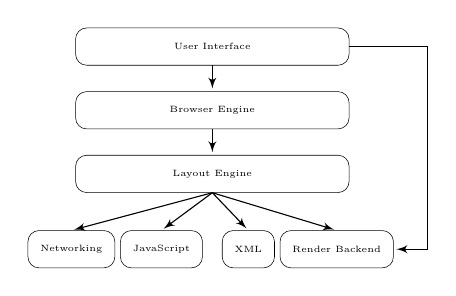
\begin{tikzpicture}[node distance=1cm, auto, transform shape, scale=0.66]  
        \tiny
          \tikzset{
              mynode/.style={rectangle,rounded corners,draw=black, top color=white, bottom color=white,very thin, inner sep=1em, minimum size=3em, text centered},
              myarrow/.style={->, >=latex', shorten >=1pt, thin},
              mylabel/.style={text width=3em, text centered}
          }  
          \node[mynode, text width=20em] (ui) {User Interface};  
          \node[mynode, text width=20em, below=0.5cm of ui] (browser-engine) {Browser Engine};
          \node[mynode, text width=20em, below=0.5cm of browser-engine] (layout-engine) {Layout Engine};
          \node[below=of layout-engine] (dummy) {};
          \node[mynode, below=of layout-engine, left=0.1cm of dummy] (javascript) {\gls{JavaScript}};
          \node[mynode, below=of layout-engine, left=0.1cm and 0.1cm of javascript] (networking) {Networking};  
          \node[mynode, below=of layout-engine, right=0.1cm of dummy] (xml) {\gls{XML}};
          \node[mynode, below=of layout-engine, right=0.1cm and 0.1cm of xml] (render-backend) {Render Backend};

          \draw[myarrow] (ui.south) -- (browser-engine.north);
          \draw[myarrow] (browser-engine.south) -- (layout-engine.north);
          \draw[myarrow] (layout-engine.south) -- (networking.north); 
          \draw[myarrow] (layout-engine.south) -- (javascript.north);
          \draw[myarrow] (layout-engine.south) -- (xml.north);
          \draw[myarrow] (layout-engine.south) -- (render-backend.north);
          \draw[myarrow] (ui.east) -- +(1.5, 0) |- (render-backend.east);
        \end{tikzpicture} 
        \medskip
        \caption{Reference \gls{browser} architecture. The data persistence system, used by the \gls{browser} engine and the user interface, has been omitted.} 
        \label{fig:browser_architecture}
      \end{figure}
      It is shown that the \gls{layout engine} is located between the \emph{\gls{browser} engine} system and the network, \gls{JavaScript}, \gls{XML} parsing, and display backend.
      The \gls{browser} engine acts as a high level interface to the \gls{layout engine}, and is responsible for providing the \gls{layout engine} with \glspl{URI} of content that should be fetched and rendered.
      Additionally, browser engines usally provide the layout engine with layout and rendering options such as user preferred font size, zoom, etc.
      The main responsibility of the \gls{layout engine} is to render the current state of the fetched \gls{hypertext} \gls{document}.
      Since \glspl{document} may (and often do) change dynamically after parsetime it is important to keep in mind that the job of the \gls{layout engine} is continuous, and is not a one time operation.
      The parsing of \gls{HTML} is also done by the \gls{layout engine} (and not in the \gls{XML} subsystem) since \gls{HTML} is less strict and reentrant.
      In short, \glspl{layout engine} perform four distinct tasks:
      \begin{enumerate}
        \item Fetch content (typically \gls{HTML}, \gls{CSS} and \gls{JavaScript}) and parse it in order to construct a \gls{DOM} tree. \todo{Explain DOM before this?}
        \item Construct a \gls{render tree} of the \gls{DOM} tree.
        \item Layout the \glspl{element} of the \gls{render tree}.
        \item Render the \glspl{element} of the \gls{render tree}.
      \end{enumerate}
      See section~\ref{sec:dom-tree} and section~\ref{sec:render-tree} for a more in depth explanation of \gls{DOM} and \glspl{render tree}.
      \Glspl{browser} can typically display multiple pages at the same time (by using tabs, multiple windows or frames) where each page has an instance of the \gls{layout engine}.
      There are four \glspl{layout engine} that the major \glspl{browser} use, as presented in table~\ref{table:layout_engines}.
      Since Blink is a recent \gls{fork} of \gls{WebKit} they have been grouped together as \gls{WebKit}-based \glspl{layout engine}.
      This results in three distinct \glspl{layout engine} to consider; \gls{WebKit}, Gecko and Trident.
      Due to Trident being closed source, only the \gls{WebKit}-based \glspl{layout engine} and Gecko will be considered in this chapter. \todo{Only this chapter or the whole thesis?}

      \begin{table}[ht]\center
        \tiny
        \begin{minipage}[t]{0.38\linewidth}
          \begin{tabular}[t]{ l l l }
            \textbf{Engine} & \textbf{Browsers} & \textbf{Share} \\
            \hline
            Blink & Chrome, Opera & 44.38\% \\
            WebKit & Safari & 17.64\% \\
            Trident & Internet Explorer & 14.96\% \\
            Gecko & Firefox & 12.83\% \\
          \end{tabular}
        \end{minipage}
        \hspace{0.1cm}
        \begin{minipage}[t]{0.42\linewidth}
          \begin{tabular}[t]{ l l l }
            \textbf{Engine} & \textbf{Browsers} & \textbf{Share} \\
            \hline
            WebKit & Safari, Chrome, Opera & 62.02\% \\
            Trident & Internet Explorer & 14.96\% \\
            Gecko & Firefox & 12.83\% \\
          \end{tabular}
        \end{minipage}
        \caption{
          The major \glspl{layout engine} and \glspl{browser} with market shares.
          The table to the right has grouped together Blink into \gls{WebKit} since it is a recent for of \gls{WebKit}.
          See section~\ref{sec:layout_engines_market_share} for more information how the market share data was gathered.}
        \label{table:layout_engines}
      \end{table}

      %The content fetching and parsing is an advanced topic by itself, but is not relevant for element queries since they impose no fundamental changes to process.
      %Also, rendering the final layout with the render backend is not affected by element queries.
      %The construction of 

      \section{Constructing DOM trees}\label{sec:dom-tree}
        \begin{metatext}
          Here a brief explanation of \gls{DOM} trees will be given, and how they are constructed.
          In order to construct a \gls{DOM} tree, the content need to be parsed which also will be covered briefly.
          This section is mainly based on \normalfont{\cite{w3c_dom,garsiel2011browsers,w3c_css21,w3c_html}}.
        \end{metatext}

        The \gls{DOM} is a convention for representing and interacting with objects in \gls{XML}-based \glspl{document} (such as \gls{HTML}).
        The \gls{DOM} provides an interface for programs (\gls{JavaScript} in the \gls{browser}) to access and mutate the structure, style, and content of \glspl{document}.
        Elements of the \gls{document} is converted to \gls{DOM} nodes, and therefore the whole \gls{document} is represented as a tree structure of \gls{DOM} nodes which is referred to as the \gls{DOM} tree.

        \Glspl{layout engine} construct \gls{DOM} trees by parsing \gls{HTML} with any included \gls{CSS} and \gls{JavaScript}.
        Parsing of \gls{HTML} is not an easy task, partly because it is expected (alhough not required) of layout engines to be forgiving of errors, such as handling malformated \gls{HTML}.
        As \gls{CSS} and JavasScript are stricter, their grammar can be expressed in a formal syntax and can therefore be parsed with a context free grammar parser.
        Another big quirk to parsing \gls{HTML} is that it is reentrant that means that the source may change during parsing, see listing~\ref{code:reentrant-html}.
        Script \glspl{element} are to be executed synchronously when it is occurred by the parser.
        If such script mutates the \gls{DOM}, then the parser will need to evaluate the changes made by the script and update the \gls{DOM} tree.
        External scripts need to be fetched in order to be executed, which halts the parsing unless the script \gls{element} states otherwise.
        It should be noted that although \gls{DOM} nodes do include a \code{style} property, the nodes in the \gls{DOM} tree are not affected by the \gls{CSS} cascading, and the style properties do not represent the final style of the \gls{element}.
        Instead, for scripts to obtain the final computed style for an \gls{element} a special function needs to be called (\code{getComputedStyle} in \gls{JavaScript}).
        Since externally linked \gls{CSS} \glspl{document} do not directly affect the \gls{DOM} tree they could conceptually be fetched and parsed after the parsing of the \gls{HTML}.
        However, scripts can request the computed style of \gls{DOM} nodes and therefore either the parsing of \gls{HTML} needs to be halted in order to fetch and parse \gls{CSS} when needed, or the scripts accessing style properties of \gls{DOM} nodes need to be halted.
        A common optimization is to use a speculative parser that continues to parse the \gls{HTML} when the main parser has halted (for executing the scripts usually).
        The speculative parser does not change the \gls{DOM} tree, instead it searches for external resources that can be fetched in parallel while waiting for the main parser to continue.

        \begin{lstlisting}[caption={Simple example of reentrant HTML. The layout engine needs to reconstruct the \gls{DOM} tree after executing the JavaScript. The page will not be rendered until all JavaScript has been executed.}, captionpos=b, label={code:reentrant-html}]
<html>
  <body>
    <div id="container">
      <p id="tip">When in doubt, mumble.</p>
    </div>
    <script>
      var container     = document.getElementById("container");
      var tip           = document.getElementById("tip");
      var intro         = document.createElement("h4");
      intro.innerHTML   = "A tip:";
      container.insertBefore(intro, tip);
    </script>
  </body>
</html>
        \end{lstlisting}

        \todo[inline]{Philipp: Yes, a picture of the DOM corresponding to some HTML would be good.}
        \todo[inline]{Figure of how the DOM tree looks like? Maybe example HTML and DOM tree figure.}
        \todo[inline]{Write about media type, and how the CSS is calculated if it is in this stage?}

      \section{Render trees}\label{sec:render-tree}
        \begin{metatext}
          When the \gls{DOM} tree has been constructed and all external \gls{CSS} has been fetched and parsed, it is time for the \gls{layout engine} to create the \gls{render tree}.
          Here an explanation of the creation process and the structure of \glspl{render tree} will be given.
          This section is mainly based on \normalfont{\cite{garsiel2011browsers,w3c_css21}}.
        \end{metatext}

        A \gls{render tree} is a visual representation of the \gls{document}.
        In contrast to the \gls{DOM} tree, the \gls{render tree} only contains \glspl{element} that will be rendered.
        The nodes of the \gls{render tree} are called \emph{renderers} (also known as \emph{frames} or \emph{render objects}), as the nodes are responsible for their own and all subnodes layout and rendering.
        In order to know how to render themselves, the final style of each renderer needs to be computed which is done by the \gls{layout engine} while constructing the tree.
        Each renderer represents a rectangle (with a size and position) with a given style.
        There are different types of renderers, which affect how the renderer rectangle is computed.
        The type can be directly affected by the \code{display} style property.

        Typically nodes of the \gls{DOM} tree has a 1:1 relation to nodes of the \gls{render tree}, but the relation can also be smaller or larger.
        The \gls{render tree} only contains nodes that will affect the rendered result, so nodes that do not affect the layout flow of the \gls{document} and that aren't visible will not be present in the \gls{render tree}.
        For instance, a \gls{DOM} node with the \code{display} property set to \code{none} will have the relation 1:0 (it will not be present in the \gls{render tree} because it is not visible and will not affect the layout flow).
        It should be noted that nodes with the \code{visibility} style property set to \code{hidden} will be present in the \gls{render tree}, although they are not visible, since they still affect the layout flow.

        Even though all style properties have been resolved for each node in the \gls{render tree} (through \gls{CSS} cascading), the renderers still do not know about the size and position of the rectangle.
        This is because some properties cannot be resolved by style cascading.
        Some properties depend on the flow of the \gls{document}, and needs to be computed through a layout.
        The layout process will resolve the final position and size of all renderers.

      \section{Style computation}\label{sec:style-computation}
        \begin{metatext}
          Both the \gls{render tree} and scripts need to be able to get the final style of an \gls{element}.
          In order to know the final style of an \gls{element}, the style for each \gls{element} must be resolved.
          Here a brief explanation of selector matching, style cascading, inheritance and rule set specificity will be given.
          \gls{CSS} property definitions will also be described.
          This section is mainly based on \normalfont{\cite{garsiel2011browsers,w3c_css21,w3c_css_style_attr}}.
        \end{metatext}

        To trace how the style of an \gls{element} was computed can be a complex task, since there are many parameters to \gls{element} style computations.
        First, styles for an \gls{element} can be defined in several places:
        \begin{enumerate}
          \item In the default styles of the \gls{browser}.
          \item In the user defined \gls{browser} style.
          \item In external \gls{CSS} \glspl{document}.
          \item In internal \gls{CSS} \code{style} tags in the \gls{document} head.
          \item In inline \gls{CSS} in the \code{style} \gls{element} attribute.
          \item In scripts modifying the \gls{element} style through the \gls{DOM} tree.
          \item In special attributes of the \gls{element} such as \code{bgcolor} (deprecated, but possible).
        \end{enumerate}
        This can be grouped into author, user and \gls{browser} styles.
        The four first items have in common that they are \emph{cascading} their style rules through \emph{selector matching}, and may define rule sets.
        Selector matching conceptually finds all \glspl{element} in the \gls{DOM} tree that matches a \gls{CSS} selector, to apply style declarations of the rule set.
        The rule sets are weighted so that if a property is assigned values by multiple rule sets the one with highest weight will be applied.
        The weighting process starts with the origin of the style:
        \begin{itemize}
          \item In case of normal rule declarations, the style weighting relation is: $browser < user < author$.
          \item Important rule declarations have the following relation: $author < user$.
        \end{itemize}
        The weighting process continues by calculating the \emph{specificity} of all rule set selectors, the higher the specificity the higher the rule set will be weighted. \todo{Explain specificity?}
        This will make rule sets with more specific selectors override rule sets with more general selectors.
        Finally, if two rule declarations have the same weight, origin and specificity the rule set specified last will win.
        Inline \gls{CSS} does not cascade since all rules given are automatically matched with the \gls{element} of the style attribute.
        However, inline \gls{CSS} is considered with highest possible specificity when performing the style cascade.
        It is important to note that the styling methods number five and six are conceptually the same, since they both alter the style property of the \gls{DOM} representation of the \gls{element}.
        The last item method deprecated, and all styles applied this way are weighted as low as possible.

        If the cascade results in no value for an \gls{element} style property, then the property can \emph{inherit} a value or have an initial value defined by the \gls{CSS} \emph{property definition}.
        Property definitions describe how the style properties should behave, see table~\ref{table:css_property_definition} for the format of property definitions.
        For instance, the \code{width} property definition states that legal values are absolute lengths, percentages or \code{auto} (which will let the \gls{browser} decide).
        The percentages are relative to the containing block.
        The initial value is \code{auto}, the properties applies to all non-replaced inline \glspl{element}, table rows and row groups.
        The value may not be inherited, and the media group is \code{visual}.
        The computed value is either the absolute length, calculated percentage of the containing block or what the \gls{browser} decides (in case of \code{auto}).
        If a property may inherit values, it will inherit the value of the first ancestor that has a value that is not \code{inherited}.

        \begin{table}[ht]\center
          \tiny
          \begin{tabular}[t]{ r | l }
            \textbf{Value} & Defines the legal values and the syntax. \\
            \textbf{Initial} & The initial value that the property will have. \\
            \textbf{Applies to} & The \glspl{element} that the property applies to. \\
            \textbf{Inherited} & Determines if the value should be inherited or not. \\
            \textbf{Percentages} & Defines if percentages are applicable, and how they should be interpreted. \\
            \textbf{Media} & Defines which media group the property applies to. \\
            \textbf{Computed value} & Describes how the value should be computed. \\
          \end{tabular}
          \caption{The \gls{CSS} property definition format that describes how all \gls{element} style properties behave.}
          \label{table:css_property_definition}
        \end{table}

        This process will resolve most style properties, but as stated in section~\ref{sec:render-tree} some properties require a layout in order to be resolved.

        \todo[inline]{How does selector matching work? Parallel?}
        \todo[inline]{Cascading, parallel?}
        \todo[inline]{Explain the syntax of CSS?}

      \section{The layout process}\label{sec:layout-process}
        \begin{metatext}
          When the \gls{render tree} has been constructed and the style properties has been resolved for all nodes, it is time to perform the actual layout.
          The layout process will decide the final computed style of all \glspl{element}, and needs to be done before rendering.
          This section will describe the layout process, discuss some performance aspects and show examples when layout happens.
          This section is mainly based on \normalfont{\cite{garsiel2011browsers}}.
        \end{metatext}

        The layout (also called \emph{reflow}) of \gls{HTML} is flow based, which means that \gls{document} layout can generally be performed top to bottom and left to right in one pass.
        This is possible because the geometry of \glspl{element} typically do not depend on the siblings or children\todo{Seems weird to say that flow is not dependent on children, since the height is propagated upwards.}.
        Layout is performed recursively by starting at the root of the tree, let the renderer render itself and all of its children which will render themselves and their children and so on.
        When a layout is performed on the whole \gls{render tree} it is called a \emph{global layout}.
        To avoid global layouts when a renderer has been changed, a dirty bit system is usually implemented.
        The system marks which renderers in the tree that need a layout, which avoids layout of unaffected \glspl{element}.
        Layouts that only layout the dirty renderers are called \emph{incremental layouts}.
        \Glspl{layout engine} that uses the dirty bit system usually keeps a queue of incremental layout commands.
        The scheduler system later triggers a batch execution of the incremental layout commands asynchronously.
        A global layout is triggered when the \gls{viewport} is resized or when styles that affect the whole \gls{document} are changed (such as \code{font-size}).
        Because the \gls{API} of \code{getComputedStyle} promises resolved values for all style properties, calling the function forces a full layout (flushing the incremental layout commands queue).
        When a renderer performs a layout the following usually happens:
        \begin{enumerate}
          \item The own width of the renderer is determined.
          \item The renderer positions all children and requests them to layout themselves (with given position and width).
          \item The heights, margins and paddings of the children are accumulated in order to decide the own height of the renderer.
        \end{enumerate}
        Of course, only the children that need a layout will be affected (dirty, or global layout) in step 2.
        So, the widths and positions are sent down in the tree and the heights are sent up in the tree in order to construct the final layout.

        The widths are calculated by the \code{width} style of the \glspl{element}, relative to the container \gls{element} width.
        Margins and paddings are also taken into account when calculating the widths.
        When the width of an \gls{element} is calculated, it needs to be controlled against the \code{min-width} and \code{max-width} style properties and make sure that the width is inside the range.
        If the content of an \gls{element} does not fit with the calculated width (text usually needs to perform line break when the width is too small), the \gls{element} needs to break up the content into multiple renderers in order to expand the height.
        The renderer that has decided it needs to break the content up into multiple renderers propagates to the parent renderer that it needs to perform the breaking.
        When the parent renderer has created the renderers needed to fit the content with the given height, layout is performed on the new renderers and then the final height can be calculated and propagated upwards.

        \todo[inline]{Are incremental layout commands really batch processed?}

      \section{Parallelization}\label{sec:parallel}
        \begin{metatext}
          No longer can performance of an application increase over time without any code changes (as opposed to the times when the \gls{CPU} clock speeds increased rapidly).
          Now, applications need to utilize the multiple cores of the \gls{CPU} instead of relying on high clock speed.
          Parallelization is something \gls{layout engine} vendors are interested in, and research is being done about utilizing multiple cores to increase the performance of the engines.
          In this section a small summary will be given about the current research front, and how the parallelization can be approached.
          This section is mainly based on \normalfont{\cite{zoomm,parallelizing_the_web_browser,meyerovich2010fast,servo_parallel,servo_blog}}.
          \todo{Check so that the section actually does what the meta says}
        \end{metatext}

        As \gls{web} applications grow bigger and more demanding, \glspl{browser} continuously need to improve the performance on all levels.
        Fetching resources over the network is the only thing that is done in parallel today.
        The rest of the \gls{browser} system is designed and optimized to run sequentially.
        On computers, \glspl{browser} usually achieve parallelism by running each page context in parallel (each tab and window of the \gls{browser} runs in a separate process).
        This approach is appealing because it utilizes the cores of the machine by still having all subsystems run sequentially for each page, while improving the overall performance of the \gls{browser}.
        However, this approach is not enough.
        The page performance is not improved if only one page is present.
        For the \gls{web} to be a true competitor to heavy native applications\todo{Reformulate to not use the word native.}, the page performance needs to be increased (not only the overall \gls{browser} performance).
        It is then important to be able to dedicate multiple cores to one page instead of having all the pages present using their own core (perhaps all non-visible pages can share one core while the main visible page can have access to multiple cores if needed).
        Also, with the number of mobile devices browsing the \gls{web} increasing rapidly it is important to be able to achieve good parallelism.
        Light devices such as small laptops, mobile phones and tablets share a common goal --- they want to reduce power consumption while increasing the performance.
        This can be achieved with multicore processors that run at lower clock speeds.
        \todo{Write that many cores is preferred over high clock speed? Why?}
        It has been shown that the performance of mobile \glspl{browser} is \gls{CPU} bound contrary to the common belief that they are network bandwidth bound \cite{parallelizing_the_web_browser}.
        This is why many researchers target light devices when trying to parallelize \gls{web} \glspl{browser}.
        Of course, once the methods has matured and been implemented, desktop layout engines will benefit from parallelization as well.

        \gls{CSS} selector matching is a good candidate for parallelization, due to matching nodes to selectors being independent from other selector matches.
        A successful parallelization of selector matching has been achieved with locality-aware task parallelism \cite{parallelizing_the_web_browser}.
        It has also been shown that selector matching and style resolving (through cascading) can be parallelized \cite{zoomm}.
        It is possible to resolve \gls{element} styles in parallel as long as two requirements are fulfilled: the matching task must have finished for the \gls{element} to resolve styles for, and the parent \gls{element} must have resolved all styles (since the \gls{element} might inherit some styles from the parent).
        As long as these requirements are fulfilled, selector matching and style resolving can run in parallel for different \glspl{element}.
        The layout process can also be parallelized, since the layout process has been shown to be sub-tree independent for non-float \glspl{element} \cite{servo_parallel,servo_blog}.
        Siblings of the layout tree can be processed independently of each other (in the general case), and is suitable to parallelize with a work stealing system.
        
        \todo[inline]{Write about the fork-join model of the parallelization as described in servo?}
        \todo[inline]{Philipp: It would be very interesting to just shortly summarize typical performance gains due to parallelization.}

    \chapter{Element queries}
      \begin{metatext}
        Now that a good understanding of \glspl{browser} (especially the \gls{layout engine}), \gls{responsive} design, and modular development has been acquired it is time to address element queries --- the solution to the modular \gls{responsive} \gls{web} design problem.
        This chapter will define element queries, present why they are needed, and address some of the issues hindering element queries from being implemented \glslink{native}{natively}.
        Further, some possible restrictions will be presented to resolve some of the \gls{native} issues.
        \todo{Instead write that some solutions will be presented?}
      \end{metatext}

      Recall from section~\ref{sec:rwd} that \gls{responsive} \gls{web} design is the concept of having \glspl{element} respond to size changes.
      \Gls{responsive} \gls{web} design implements this by using \gls{media queries}, applying conditional rules with relation to the \gls{viewport} size.
      In section~\ref{sec:modularity} the desire for building modular \gls{web} components was presented.
      One positive outcome of building applications in a modular way is that general components become reusable.
      Since the only way of applying conditional rules to \glspl{element} today is by using \gls{media queries}, all \gls{responsive} styles must be defined by the application and not by the modules (because only the application knows how much space each module will be given in the application layout).
      The implication of this is that the \gls{HTML} and \gls{JavaScript} can be written in a modular way, but the \gls{CSS} is left for the user of the module (application) to write which somewhat defeats the purpose of writing modules.
      So developers today have two choices: writing modules that are not \gls{responsive} but \gls{self-contained}, or writing modules that are \gls{responsive} but not \gls{self-contained} (leaving the styling to the user).

      The solution to this is element queries, which allows conditional rules to be applied based on any criteria for any \gls{element}.
      Figure~\ref{fig:mq-vs-eq} shows the problem with \gls{media queries} and the element query solution.
      The typical use case is to write conditional styles to be applied based on the container \gls{element} size.
      Although the size of the container \gls{element} is typically the most interesting element query with \gls{responsive} \gls{web} design, element queries as a concept does not need to be limited to that.
      It is also possible to apply conditional rules by any \gls{element} display property, color, text alignment, and so on.
      Theoretically it should be possible to query any style property of an \gls{element}, but the focus will be the \code{width} and \code{height} properties since they are the most interesting in \gls{responsive} \gls{web} design.

      \begin{figure}
        \centering
        \begin{minipage}{.5\textwidth}
          \centering
          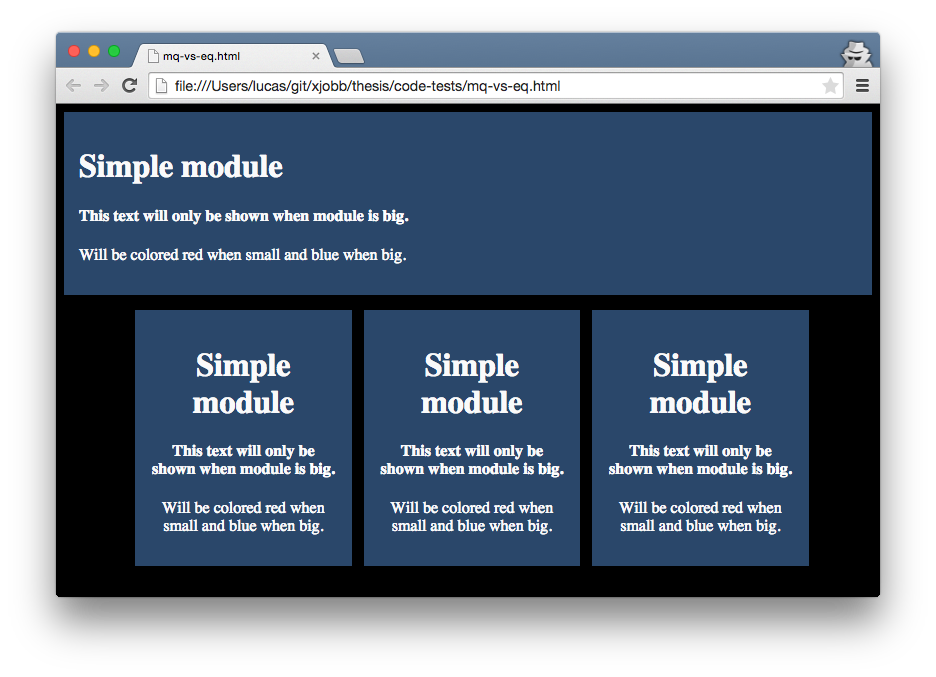
\includegraphics[width=\linewidth]{images/mq-big}
        \end{minipage}%
        \begin{minipage}{.5\textwidth}
          \centering
          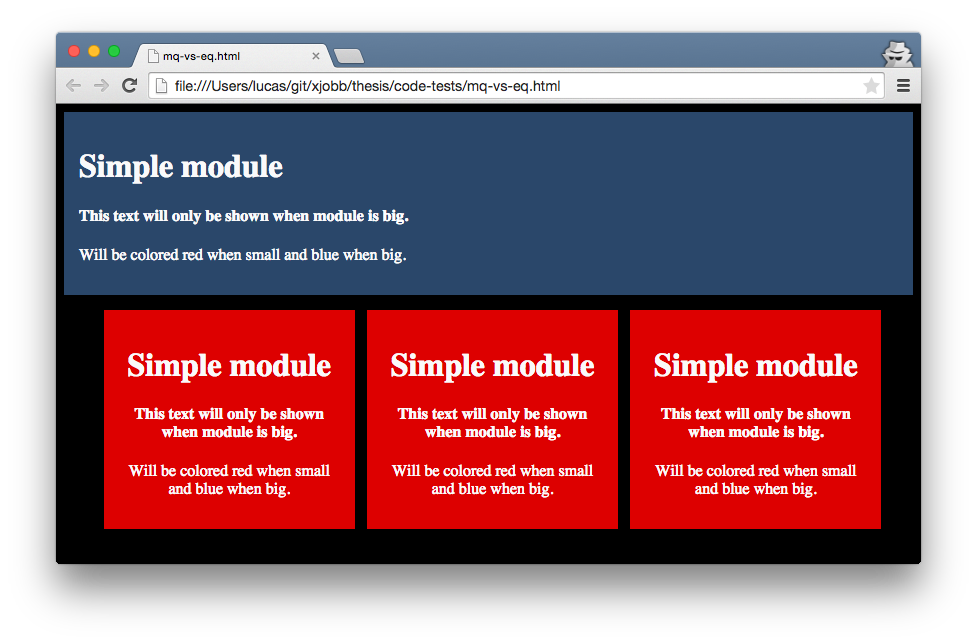
\includegraphics[width=\linewidth]{images/eq-big}
        \end{minipage}
        \caption{
          The problem of \gls{media queries} and the element query solution.
          Both images shows four instances of a module in different sizes.
          The module is \gls{responsive}, so when it is small it should change color to red and change the inner text a bit.
          The left version is built with \gls{media queries}; hence all module instances stay blue even though some are small (only a smaller \gls{viewport} will trigger the modules to change style).
          The right version is built with element queries, hence the modules display differently depending on the given size that each module has, which is the desired behavior.}
        \label{fig:mq-vs-eq}
      \end{figure}

      \section{Problems}
        \begin{metatext}
          The main reason why element queries have not been implemented \glslink{native}{natively} in \glspl{browser} is because they bring problems and limitations to the \glspl{browser}.
          It is important to understand the problems in order to speculate about a potential \gls{native} \gls{API} design.
          In this section the two major problems will be presented; performance and circularity.
        \end{metatext}

        \todo{What to write here?}
        \subsection{Performance}
          \begin{metatext}
            This subsection will present the performance impacts that element queries have on \glspl{layout engine}.
            As shown in section~\ref{sec:parallel} \gls{layout engine} vendors are interested in parallelizing their engines to increase the page performance.
            Element queries limits the parallelization, which will be the focus of this subsection.
            This subsection is partly based on \normalfont{\cite{w3c_eq_mail}}.
            \todo{Referera till w3c mailinglista?}
          \end{metatext}

          Recall from section~\ref{sec:layout-process} that the rectangle size and position for each \gls{element} is calculated in the layout process, and cannot be determined before an actual layout has happened.
          This imposes that a layout pass needs to be performed before knowing the \gls{element} sizes.
          If element queries are present that rely on the size of \glspl{element}, which is the identified common use case, the following process needs to happen:
          \begin{enumerate}
            \item A layout pass needs to be performed in order to calculate the size of the \glspl{element} targeted by element queries.
            \item The element query conditional rules need to be evaluated against the \glspl{element} to know which rules should be applied (element query selector matching).
            \item If the element query selector matching has resulted in a different matching set than in step 1, the process is repeated (with the new rules applied).
          \end{enumerate}
          So, an element query selector matching change result in performing another layout, discarding at least a subtree of the previous layout.
          As already stated, this only occurs when the layout has changed in a way that changes the element query selectors.
          Unfortunately, this means that if there is any matching element query selector at page load, two layout passes will always be performed.

          Further, it is common for internal \glspl{API} in \glspl{layout engine} to request updated \gls{element} styles that do not require layout to resolve (non-layout properties such as \code{color} and \code{font-family}).
          Since a layout of the element query selector target is required in order to resolve the correct \gls{element} style, such internal \glspl{API} requires a layout in order to obtain the correct \gls{element} style (even for non-layout related properties).
          Also, \glspl{layout engine} would not be able to layout subtrees in parallel since an \gls{element} in one subtree might affect an \gls{element} in another subtree.

          \todo{Totally forgot to write about parallel problems}

        \subsection{Circularity}\label{sec:cyclic-rules}
          \begin{metatext}
            This subsection will show how cyclic rules may occur and why it is a problem.
            It will also be presented why cyclic rules must be detected at runtime.
            Some examples will be given to better understand the complexity of the problem.
          \end{metatext}

          The most obvious occurrences of cyclic rules are when there are specified conflicting width element queries and width updates for an \gls{element}.
          See listing~\ref{code:cyclic-simple} for the perhaps simplest example of cyclic rules.
          The syntax of element queries will be presented in section~\ref{sec:native-eq}\todo{Have the explanation before this section? On the other hand this section is needed for the motivation of the syntax of the native API}, and is not important to understand the problem.
          \begin{lstlisting}[caption={Simple example of cyclic rules with directly conflicting width element queries and updates.}, captionpos=b, label={code:cyclic-simple}]
#foo {
  width: 250px;
}

#foo:eq(max-width: 300px) {
  /* This rule will be applied only when the width of #foo is <= 300px. */
  width: 550px;
}

#foo:eq(min-width: 500px) {
  /* This rule will be applied only when the width of #foo is >= 500px. */
  width: 250px;
}
          \end{lstlisting}

          The following happens to the \gls{element}:
          \begin{enumerate}
          \item The initial width of the \code{\#foo} \gls{element} is set to 250 pixels.
          After a layout, the \code{\#foo:eq(max-width: 300px)} matches and therefore next step will be 2.
          \item The width of the \gls{element} is under 300 pixels, so the selector \code{\#foo:eq(max-width: 300px)} matches.
          Note that the \code{\#foo:eq(min-width: 500px)} does not match, since the width is under 500 pixels.
          Since the matched selector is more specific than the \code{\#foo} selector, the new width of the \gls{element} is 550 pixels.
          Next step will be 3.
          \item The width of the \gls{element} is above 500 pixels, so the selector \code{\#foo:eq(min-width: 500px)} matches.
          Note that the \code{\#foo:eq(max-width: 300px)} does not match, since the width is above 300 pixels.
          Since the matched selector is more specific than the \code{\#foo} selector, the new width of the \gls{element} is 250 pixels.
          Next step will be 2.
          \end{enumerate}
          Clearly, the \gls{browser} will be stuck in an infinite layout cycle pending back and forth between step 2 and 3 (250 pixels and 550 pixels).
          The result of this is of course implementation dependent.
          One reasonable outcome of such infinite layout loop is that the \gls{layout engine} executes one layout pass and then evaluate the next set of matched selectors and so on, which leads to a functioning page but since a relayout is enforced every update, the performance impact is huge.
          This example is somewhat similar to writing \code{while(true);} in \gls{JavaScript}, which obviously is a bad idea.
          However, cyclic rules can also occur in less obvious ways. 

          Indirect cyclic rules are somewhat more complex to reason about, than the example given above (which is an example of direct cyclic rules).
          For instance, if the \code{\#foo} \gls{element} matches the width of a child \gls{element}, and the child changes width depending on the parent width, a cycle might occur.
          Consider the code in listing~\ref{code:cyclic-2}.
          
          \begin{lstlisting}[caption={Example of indirect cyclic rules. Here the user (\code{\#foo}) of the module (\code{\#module}) creates cyclic rules indirectly by specifying that it should match the width of the module.}, captionpos=b, label={code:cyclic-2}]
/* HTML */
<div id="foo">
  <div id="module">
    <div id="child"></div>
  </div>
</div>

/* CSS */
#foo {
  /* Will match the width of the child element #module. */
  display: inline-block;
}

#module {
  /* Matches the width of the parent element #foo. */
  width: 100%;
}

#child {
  width: 250px;
}

#module:eq(max-width: 300px) #child {
  /* This rule applies only when the width of #module is <= 300px. */
  width: 550px;
}

#module:eq(min-width: 500px) #child {
  /* This rule applies only when the width of #module is >= 500px. */
  width: 250px;
}
          \end{lstlisting}
          What makes this situation more complex than the previous example is that it is less obvious for the devloper to identify that there are cyclic rules.
          First, the problem cannot be found without considering the rule sets of both the module and the \code{\#foo} element.
          Second, the rules of the module elements and the rules of the \code{\#foo} \gls{element} might be separated into different parts of the stylesheet or different stylesheets.
          Third, the user of the module must be aware of how it styles itself in order to understaind the limitations it imposes.
          By adding adding one line to the containg element \code{\#foo} a cycle appears in another part of the program (in the module).
          A \gls{JavaScript} quivalent of this example would perhaps be \code{var bar = true; while(bar);} with the motivation that it is still obvious that it results in an infinite loop but both the loop and the variable needs to be considered.
          Also, the variable assignment could happen in another part of the program.

          The examples given so far have been simple, and can easily be identified as cyclic by reviewing the \gls{CSS} code.
          It would also be possible for a static analyzer to detect the cycles. \todo{Write at parse time instead of static analyzer?}
          However, cycles can occur in a complexer way that cannot be detected by a static analyzer.
          Consider the code in listing~\ref{code:cyclic-3}.
          \begin{lstlisting}[caption={Example of cyclic rules that cannot be detected by a static analyzer.}, captionpos=b, label={code:cyclic-3}]
/* HTML */
<span id="foo">
  When in doubt, mumble.
</span>

#foo:eq(max-width: 300px) {
  /* This rule applies only when the width of #foo is <= 300px. */
  font-size: 2em;
}
          \end{lstlisting}
          In this example, it is virtually impossible to tell if the rules are cyclic for a static analyzer.
          It could perhaps guess that it could result in a cycle in some cases but that is also the point of the example --- it is only cyclic in some scenarios.
          The size of the \code{\#foo} element will depend on the content of it (i.e, the text).
          The width of the text depends on the font size, which is inherited.
          So the width of the \code{\#foo} \gls{element} is dependent on the inherited font size.
          When the \code{\#foo} \gls{element} is below 300 pixels wide, the font size of the element is increased to \code{2em} (which is a unit that is relative to the inherited value).
          If a \code{2em} font size results in a computed font size big enough to make the \gls{element} wider than 300 pixels, the \code{\#foo:eq(max-width: 300px)} selector will not match and therefore the element will no longer have font size \code{2em}.
          Since the element width is decreased below 300 pixels when the font size of \code{2em} no longer is applied, the selector will match again --- the rules are cyclic.
          However, in another scenario the inherited font size might not be big enough to make the \code{\#foo} element wider than 300 pixels which would not result in a cycle.
          The factors that creates the cycle are the following:
          \begin{itemize}
            \item The display type of the \gls{element}
            \item The \gls{element} queries of the \gls{element}
            \item The font size value of the \gls{element}
            \item \textbf{The inherited font size of the \gls{element}}
            \item \textbf{The content of the \gls{element}}
          \end{itemize}
          The factors in bold are of a far worse type than the ones presented.
          They are impossible to determine at parsetime.
          In this example the text is static but it could have been added dynamically.
          Also, the inherited font size value on the closest ancestor with a font size property defined.
          Since ancestors also can have their font sizes defined in relative units, the dependency tree can go up to the root of the \gls{document}.
          Further, if no ancestor defines an absolute value for the font size it is up to the \gls{browser} to default to a size, which is impossible to reason about at parsetime.
          This implies that there is no way of telling if the cycle appears or not without actually running the code.
          Also, the cycle may appear in different \glspl{browser} and settings, which makes the cycle even harder to detect.\todo{Also write that it depends on the content, which might not be present at parsetime.}
          Far worse is that the previous examples have been of the \code{while(true);} character, which gives the false hope that even though it is possible to create cycles developers would never encounter it since ``real'' code would not be close to the examples given here. \todo{Thinking about removing this... This does not seem like a valid use case, since the layout area is depending on the content.}
          With the third example, this is no longer true.
          Increasing the font size when the layout area is smaller and decreasing the font size when the layout area is bigger is something that is frequently done in \gls{responsive} \gls{web} design.
          Typically \gls{web} site authors want the font size to increase on handheld devices, to increase the readability.
          Of course, the numbers given in the example might not be reasonable, but in concept it is valid use case that may result in cyclic rules.

      \section{Possible solutions}
        \begin{metatext}
          Now that the problems of element queries have been presented, it is time to show some possible solutions to the problems.
          The different solution approaches either limits element queries in some way or solves only a subproblem, so no perfect solution that keeps element queries unlimited with decent performance has been found.
        \end{metatext}

        \todo{Write somewhere that iframes are not a solution? But they are close to a solution...}
        \subsection{Viewport elements}\label{sec:viewport-elements}
          \begin{metatext}
            This solution limits element queries a lot, but avoids many of the problems this way.
            This approach has been discussed at the \gls{W3C} and the \gls{RICG} assumes that this is a prerequisite to a \gls{native} implementation.
            \todo{cite where this has been gathered from?}
          \end{metatext}

          By limiting element queries to special \gls{viewport} container \glspl{element} that can only be queried by child \glspl{element}, much of the problems are resolved.
          This means that a new \gls{HTML} tag will be crafted (perhaps named \code{viewport}) that defines separated \glspl{viewport} in the \gls{document}.
          The size of \glspl{viewport} is not dependent on their children, and children may only target the closest ancestor \gls{viewport} \gls{element} in the element queries.
          This way, cyclic rules can no longer occur since the children may not alter the \gls{viewport} size.
          The reason that a new \gls{HTML} tag is proposed instead of a new \gls{CSS} property that defines the behavior is because the \gls{layout engine} in the latter case needs to resolve the styles for all \glspl{element} in order to know which are \gls{viewport} \glspl{element}.
          With a new \gls{HTML} tag, the \gls{layout engine} can detect that that the \gls{element} is a \gls{viewport} before any resolving styles.
          \todo{Write why it is important to know viewport elements before resolving styles.}

          This approach also solves many of the performance problems, but not all.
          The internal \glspl{API} that request non-layout information for the \glspl{element} using element queries only need to make sure that the containing \gls{viewport} \gls{element} has been laid out before resolving the styles (which is a much better situation that the unrestricted version of element queries).
          Further, the layout can be done in one pass as long as the \gls{viewport} \glspl{element} are laid out before the children.
          It is still a bit inconvenient that the \gls{layout engine} would need to evaluate all element query selectors in the middle of a layout pass (after the that the \gls{viewport} \glspl{element} has been laid out) in order to resolve the styles for the \gls{viewport} children.
          Parallelization is also easier, since the queries may only be targeting the closest \gls{viewport} \gls{element}.
          This means that each \gls{viewport} subtree can be laid out in parallel.

          This solution would behave much like the \code{iframe} \gls{element} layout-wise.
          It should be noted that \code{iframe} \glspl{element} are not suitable as an alternative to the proposed \code{viewport} \gls{element}, since \code{iframe} elements are much more limited by nature (creates a new \gls{document} and script context).

          Obviously, this limits element queries a lot.
          The fact that the size of the \gls{viewport} \gls{element} cannot depend on the children (like normal block \glspl{element} do), limits the usability.
          The idea is that the \gls{viewport} cannot be queried for properties that the children may affect (such as the width and height style properties).
          In order to allow the children to query the properties, they cannot be affected by the children.
          In theory it should mean that if no children query for instance the height of the \gls{viewport}, then the \gls{viewport} may depend on the children for it's height.
          This is a powerful insight, since the general use case would be to write element queries against the width and have the \glspl{element} adapt their heights accordingly (including the \gls{viewport} \gls{element}).
          \todo{Back this up. Maybe check with RICG if this is possible?}

        \subsection{Element queries with runtime checks}
          \begin{metatext}
            This solution does not limit element queries, but does also not solve all problems.
            Instead of making cyclic rules impossible, a mechanism to handle the cyclic rules is desired.
            Unfortunately this does not improve the performance at all, which is a major drawback.
          \end{metatext}

          \todo[inline]{Should this be incorporated with some other section or be written?}
          \todo[inline]{Maybe write about having a third-party framework as a solution?}
      \section{Native API design}\label{sec:native-eq}
        \begin{metatext}
          In this section a possible \gls{native} element query \gls{API} will be presented.
          This is based on the current information and approaches of the \gls{W3C} and the \gls{RICG}, and should therefore be regarded as a guideline of the shape of a potential standardized \gls{API}.
          \todo{Is guideline the right word? Seems a bit too confident. Also, cite here the sources of the information this section is based on?}
        \end{metatext}

        As presented in subsection~\ref{sec:viewport-elements}, \gls{viewport} \glspl{element} solve many of the element query problems and are therefore assumed to be a part of a \gls{native} \gls{API}.
        Since it would be favorable to be able to specify multiple conditional rule sets for the element queries (like \gls{media queries}) the \gls{CSS} syntax may be of the form as presented in listing~\ref{code:mq-eq-syntax}.
        \begin{lstlisting}[caption={Element queries are assumed to have nested rule sets, like \gls{media queries}},captionpos=b,label={code:mq-eq-syntax}]]
/* Media query syntax */
@media ... {
  p {
    color: red;
  }
}

/* Element query syntax */
... {
  p {
    color: red;
  }
}
        \end{lstlisting}

        \todo{Continue this if possible?}
  \part{Third-party framework}\label{part:framework}
    \todo[inline]{Write somewhere that it might be an option to not have a resize detection system, but instead let the user manually check the elements when they may have changed.}
    \todo[inline]{Write about the simple cycle detector.}
    \todo[inline]{Write about the N layouts, and how it was fixed with the batch processing. Investigate how this behaves for nested elements.}
    \todo[inline]{Write about the drawbacks (invalid layout at page load, injecting objects is heavy, DOM is mutated.)}

    \chapter{Analysis of approaches}
      \section{Current implementations}
        \todo[inline]{Write about GSS, Tommy's implementation and the different approaches}
        \todo[inline]{Write somewhere that an extra layout on elements resize is inevitable since it is required in theory.}
    \chapter{Framework design}
      \begin{metatext}
        Before starting the actual implementation, it is important to have an overall design to follow.
        In this chapter, the framework design will be described and a motivation why the framework should be plugin based will be given.
        The subsystems of the framework and their interactions will also be presented.
      \end{metatext}

      First of all, a working name of the framework needs to be established --- the framework will from now on have the working name \abbr{elq}.
      This name serves as a prefix for many of the framework \glspl{API}, and will be frequently used in the report from now on.
      The technical goals of \abbr{elq} will be stated in section~\ref{sec:techincal-goals}.
      In section~\ref{sec:arcithecture} the architecture will be described, and the subsystems of \abbr{elq} will be presented.
      Last, the \gls{API} will be defined in section~\ref{sec:elq-api}.

      \section{Technical goals}\label{sec:techincal-goals}
        \begin{metatext}
          Before presenting the overall design of the framework, the technical goals will be stated.
          It will be shown that the goals and use cases can vary from case to case, which will be the main argument to why the framework should be plugin based.
        \end{metatext}

        Expectations and requirements of element queries vary greatly by use cases.
        As usual in software development, tradeoffs need to be made.
        Some projects value simplicity and ease of use, while other projects demand advanced features and high performance.
        The requirements can be grouped into four categories; features, ease of use, performance and compatibility.
        Identified possible requirements of the framework are the following:
        \begin{enumerate}
          \item \textbf{Features}
            \begin{enumerate}
              \item\label{itm:req_resize_detect} The framework needs to augment \gls{native} element queries in the sense that styles are applied automatically on \gls{element} resizes.
              \item Existing modules written with \gls{media queries} should be automatically converted to element queries so that existing third-party modules can be used in element query empowered applications.
              \todo{Remove this?}
              \item The features should be flexible and not limited to only the common use cases.
            \end{enumerate}
          \item \textbf{Ease of use}
            \begin{enumerate}
              \item\label{itm:req_big_rewrite} Developers should not need to perform big rewrites of their modules or applications in order to use the framework.
              \item\label{itm:natural} The \glspl{API} need to feel natural and should not seem alien to \gls{web} developers.
              \item The framework should help identifying cyclic rules and prevent them from causing infinite layouts.
            \end{enumerate}
          \item \textbf{Performance}
            \begin{enumerate}
              \item The framework needs to have adequate performance to empower heavy applications running on light devices.
              \item The framework load time needs to be kept low.
            \end{enumerate}
          \item \textbf{Compatibility}
            \begin{enumerate}
              \item Older \glspl{browser} must be supported.
              \item The framework may not require invalid \gls{CSS}, \gls{HTML} or \gls{JavaScript}.
              \item\label{itm:assumption} Dependencies and assumptions about the host application (including the development environment) should be kept low.
              \item\label{itm:req_prolyfill} The framework must act as a prolyfill\footnote{A polyfill is something that provides a functionality that is expected to be provided \glslink{native}{natively} by \glspl{browser}. Polyfills usually fixes some standard functionality for \glspl{browser} that do not yet support it. A prolyfill is a polyfill for something that will probably become a standard.} for \gls{native} element queries.
            \end{enumerate}
        \end{enumerate}
        It would be possible to create a framework that conforms to all of the requirements but added features, automation and compatibility most probably would decrease the performance and load time.
        In the same way, too many advanced features may decrease the ease of use and simplicity of the \gls{API}.
        Some feature may also restrict the compatibility.
        Trying to conform to all of the requirements and trying to find a balance would result in a worse solution than a framework tailored for specific requirements.
        By providing a good framework foundation and plugins for different use cases it is up to developers to choose the right plugins for each project.
        This way, developers are composing their own custom tailored solution for their specific use cases.
        In addition, by letting the plugins satisfy the requirements it is easy to extend the framework with new plugins when new requirements arise.
        For instance, the requirement~\ref{itm:req_prolyfill} is beneficial to satisfy with a plugin since the \gls{API} for \gls{native} element queries can only be guessed at this point of time, which will probably lead to frequent changes to the plugin.
        By separating it from the core framework (and the other plugins), only developers that really desire the prolyfill behavior must handle the rapid \gls{API} changes.

      \section{Architecture}\label{sec:arcithecture}
        \begin{metatext}
          As it has been shown that a plugin based framework is suitable, it is time to present the overall architecture of the framework.
          The roles of each subsystem of the core framework will also be explained.
        \end{metatext}

        \todo[inline]{Here the style state of the element is talked about. Maybe this should have been mentioned before? Perhaps in the chapter text?}

        To decide if a subsystem of the solution should be in the framework core or a plugin is a difficult task.
        A balance needs to be found between ease of use, performance and extendability.
        All subsystems of the core need to provide a fundamental functionality to the framework and also need to be general enough to be used by plugins in different ways.
        If a plugin needs to write a custom version of a subsystem in the core in order to work, the subsystem should perhaps not be part of the core.
        Each subsystem added to the core will impact the performance negatively (by slower load time in the best case) for all users, so they must impose a real value to existing and future plugins.
        The subsystems of the core always have the risk of being redundant, unnecessary and in other ways unwanted for some use cases.
        Therefore it is important that it is possible for developers to either remove them or change them.
        This way the more advanced users can choose which subsystems to alter, keeping the framework easy to use for the common use cases.

        \begin{figure}
\centering
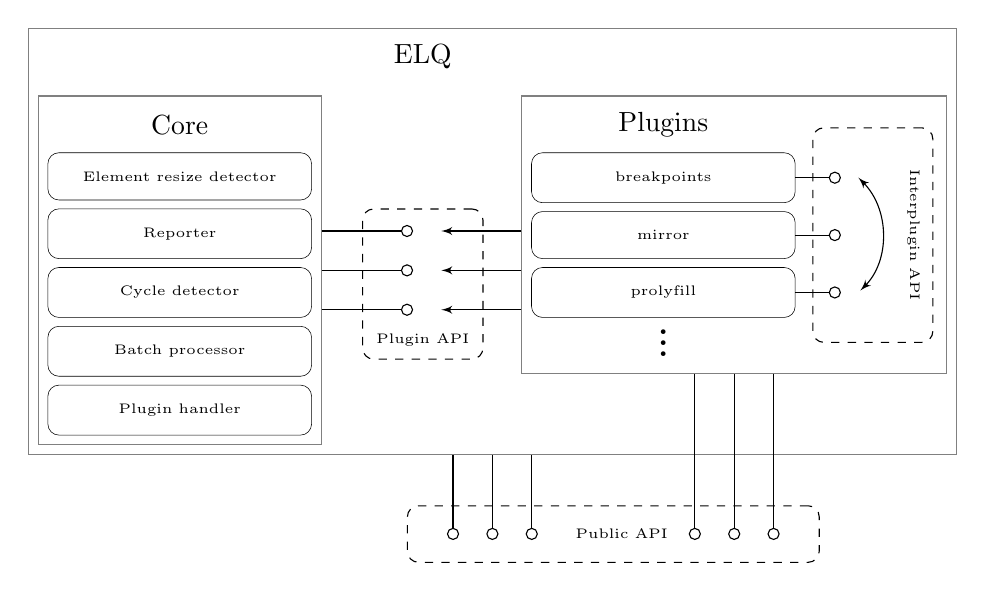
\begin{tikzpicture}[node distance=3pt]  
\tiny
  \tikzset{
      insidenode/.style={
        rectangle,
        rounded corners,
        draw=black,
        top color=white,
        bottom color=white,
        very thin,
        inner sep=1em,
        minimum height=2em,
        text centered,
        text width=12em
      },
      title/.style={
        draw=none,
        fill=none,
        top color=white,
        bottom color=white,
        thin,
        inner sep=0,
        minimum height=2em,
        text centered
      },
      box/.style={
        draw=black!50,
        inner sep=0.5em
      },
      o/.style={
        shorten >=#1,
        decoration={
          markings,
          mark={
            at position 1
            with {
              \draw circle [radius=#1];
            }
          }
        },
        postaction=decorate
      },
      o/.default=2pt,
      apibox/.style={
        minimum height=3em,
        dashed,
        draw=black,
        rounded corners
      },
      myarrow/.style={->, >=latex', shorten >=1pt, thin},
      mylabel/.style={text width=3em, text centered}
  }

  \node[] (middledummy) {};
  \node[title, above=15pt of middledummy] (elqtitle) {\normalsize ELQ};

  \node[title, left=11em of middledummy] (coretitle) { \normalsize Core };
  \node[insidenode, below=of coretitle] (erd) {Element resize detector};  
  \node[insidenode, below=of erd] (reporter) {Reporter};
  \node[insidenode, below=of reporter] (cycle) {Cycle detector};
  \node[insidenode, below=of cycle] (batch) {Batch processor};
  \node[insidenode, below=of batch] (plugin) {Plugin handler};

  \node[box, fit={(coretitle) (erd) (reporter) (cycle) (batch) (plugin)}] (core) {};

  \node[title, right=10em of middledummy] (pluginstitle) { \normalsize Plugins };
  \node[insidenode, below=of pluginstitle] (breakpoints) {breakpoints};
  \node[insidenode, below=of breakpoints] (mirror) {mirror};
  \node[insidenode, below=of mirror] (prolyfill) {prolyfill};
  \node[below=-4pt of prolyfill] (dots) {\huge \vdots};
  \node[box, fit={(pluginstitle) (breakpoints) (mirror) (prolyfill) (dots) ($ (breakpoints.east) + (1.8,0) $)}] (plugins) {};

  \node[box, fit={(elqtitle) (core) (plugins)}] (elq) {};

  % Interplugin API
  \draw[o] (breakpoints.east) -- ($ (breakpoints.east) + (0.5,0) $);
  \draw[o] (mirror.east) -- ($ (mirror.east) + (0.5,0) $);
  \draw[o] (prolyfill.east) -- ($ (prolyfill.east) + (0.5,0) $);
  \draw[myarrow, <->] ($ (breakpoints.east) + (0.8,0) $) to[out=-45, in=45] ($ (prolyfill.east) + (0.8,0) $);
  \node[mylabel, rotate=-90, text width=10em] (interpluginapilabel) at ($ (mirror.east) + (1.5,0) $) {Interplugin \gls{API}};
  \node[apibox, fit={($ (breakpoints.east) + (0.3,0.5) $) ($ (prolyfill.east) + (0.3,-0.5) $) (interpluginapilabel)}] (interpluginapi) {};

  % Public API
  \coordinate (pubapibottom) at ($ (elq.south) + (0,-1) $);
  \draw[o] ($ (elq.south) + (0,0) $) -| (pubapibottom);
  \draw[o] ($ (elq.south) + (-0.5,0) $) -| ($ (pubapibottom) + (-0.5,0) $);
  \draw[o] ($ (elq.south) + (0.5,0) $) -| ($ (pubapibottom) + (0.5,0) $);
  \draw[o] let \p1=(pubapibottom), \p2=(plugins.south) in ($ (plugins.south) + (0,0) $) -| ($ (\x2,\y1) + (0,0) $);
  \draw[o] let \p1=(pubapibottom), \p2=(plugins.south) in ($ (plugins.south) + (0.5,0) $) -| ($ (\x2,\y1) + (0.5,0) $);
  \draw[o] let \p1=(pubapibottom), \p2=(plugins.south) in ($ (plugins.south) + (-0.5,0) $) -| ($ (\x2,\y1) + (-0.5,0) $);
  \node[mylabel, right=4em of pubapibottom, text width=5em] (pubapilabel) {Public \gls{API}};
  \path let \p1=(pubapibottom), \p2=(plugins.south) in node (pubapiright) at ($ (\x2,\y1) + (0.5,0) $) {};
  \node (pubapileft) at ($ (pubapibottom) + (-0.5,0) $) {};
  \node[apibox, fit={(pubapibottom) (pubapilabel) ($ (pubapileft) + (-0.5,0) $) ($ (pubapiright) + (0.5,0) $)}] (publicapi) {};

  % Plugin API
  \path let \p1=(middledummy.south), \p2=(core.east) in coordinate (pluginapi) at (\x1, \y2);
  \node[mylabel, below=3em of pluginapi, text width=5em] (pluginapilabel) {Plugin \gls{API}};
  \draw[o] ($ (core.east) + (0,0) $) -- ($ (pluginapi) + (-0.2,0) $);
  \draw[o] ($ (core.east) + (0,0.5) $) -- ($ (pluginapi) + (-0.2,0.5) $);
  \draw[o] ($ (core.east) + (0,-0.5) $) -- ($ (pluginapi) + (-0.2,-0.5) $);
  \draw[myarrow] let \p1=(core.east), \p2=(plugins.west) in ($ (\x2, \y1) + (0,0) $) -- ($ (pluginapi) + (0.2,0) $);
  \draw[myarrow] let \p1=(core.east), \p2=(plugins.west) in ($ (\x2, \y1) + (0,0.5) $) -- ($ (pluginapi) + (0.2,0.5) $);
  \draw[myarrow] let \p1=(core.east), \p2=(plugins.west) in ($ (\x2, \y1) + (0,-0.5) $) -- ($ (pluginapi) + (0.2,-0.5) $);
  \node[apibox, fit={(pluginapilabel) ($(pluginapi) + (0, 0.7)$)}] (pluginapibox) {};
\end{tikzpicture}
\medskip
\caption{
  The overall library architecture, which shows how the library is divided into two parts; the core and plugins. 
  The core is generally only accesible through the plugin \gls{API}, and is not a part of the public \gls{API}.
  Plugins may have interplugin \glspl{API} and dependencies.
  The bigger part of the public \gls{API} is defined by the plugins.
}
\label{fig:elq_architecture}
\end{figure}

        Figure~\ref{fig:elq_architecture} shows the overall architecture of the framework.
        The core consists of fundamental and general subsystems that are utilized by plugins.
        Developers should never be programming against the core directly, and it can therefore only be accessed by plugins through the hidden plugin \gls{API}.
        The framework provides a small public \gls{API} which is mainly used to invoke and handle plugins.
        The plugins form the bigger part of the public \gls{API} in the sense that they decide which features exist and how they work.
        It should be noted that plugins may provide \glspl{API} through the framework by registering methods, or by specifying custom syntax (such as markup or \gls{CSS}) which is beyond the control of the core.
        Plugins may also have interplugin \glspl{API} and dependencies, which also is beyond the control of the core.
        The core is supposed to have a slow development phase, with few changes and good backwards compatability.
        Plugins may be developed in a high rate, with frequent changes to support new features.
        Subsystems that are part of the core are the following:
        \begin{itemize}
          \item \textbf{Reporter:}
            Responsible for reporting information, warnings and errors to the developer.
            By having a centralized reporter, it is possible to decide at a global framework level how much plugins are allowed to report.
            Other options such as throwing exception on errors or warnings could also be set at a global framework level.
            Also, the framework can make sure that all reports are standardized and can provide extra information such as the name and version of the plugin along with its report.
            To avoid code duplication, it also beneficial to have a centralized report system so plugins do not need to perform the same compatibility checks (such as checking if the \gls{browser} actually supports console reporting).
          \item \textbf{Element resize detector:}
            Provides an interface for listening to \gls{element} resize events.
            This system is fundamental to plugins fulfilling requirements \ref{itm:req_resize_detect} and \ref{itm:req_big_rewrite} since it enables the framework to be aware of when \glspl{element} change sizes, instead of the host application keeping track of when \glspl{element} have changed sizes.
            \todo[inline]{Maybe this shouldn't be a core subsystem? Since this system imposes the biggest performance impact. It might make more sense to have this as a plugin.}
          \item \textbf{Cycle detector:}
            As shown in section~\ref{sec:cyclic-rules} cyclic rules need to be detected at runtime.
            When a plugin wish to update the size state of an \gls{element} (which in turn applies the conditional styles) it can ask this system if the update seems to be part of a cycle.
            If the update seems to be part of a cycle, it is up to the plugin how that should be handled.
            \todo[inline]{Write that this system is more general, and could potentially be used for detecting other cyclic behaviors?}
          \item \textbf{Batch processor:}
            To avoid layout thrashing, it is important to read and mutate the \gls{DOM} in separate batches.
            This subsystem provides an interface for plugins to store functions to later be executed in a batch.
            To avoid layout thrashing by other scripts it can beneficial to asynchronously postpone the batch until the next layout cycle of the \gls{browser}, which is also handled by the subsystem.
          \item \textbf{Plugin handler:}
            Of course, having plugins requires a subsystem for handling them.
            This system provides the interface for developers to add plugins to the framework.
            The system is also responsible for retrieving the plugins, and invoking them on different framework events.
        \end{itemize}
        Some of the subsystems may be partially accessible through the public \gls{API} such as the plugin handler and the \gls{element} resize detector.
        It should be noted that the presented core subsystems are not the only things that the framework consists of, but the presented systems are the major ones.
      \section{API design}\label{sec:elq-api}
        \begin{metatext}
          This section will describe the \gls{API} of the framework.
          First, the public \gls{API} of the core will be presented, followed by the plugin \gls{API}.
          After that, all plugins will be described in depth addressing their features, dependencies and \glspl{API}.
        \end{metatext}

        Recall from section~\ref{sec:arcithecture} that the bigger part of the public \gls{API} is provided by plugins.
        The role of the framework is to provide plugins with systems to be used for performing element query tasks, which is done through the plugin \gls{API}.
        Three plugins will be developed; \code{breakpoints}, \code{mirror} and \code{prolyfill}.
        The \code{breakpoints} plugin provides 

        \subsection{Public API}\label{sec:public-api}
          \todo[inline]{Write how to install it. AMD, script, commonjs, etc.}
          \todo[inline]{Move getPlugin to Plugin API and make use return the plugin instance}

          In section~\ref{sec:techincal-goals} it was determined that advanced users must be able to change the subsystems used in the core.
          Therefore no global framework instance will be instantiated automatically on load.
          Instead, a function \code{Elq} that creates \abbr{elq} instances is provided in order to be able to inject dependencies.
          The function accepts an optional options object parameter, where it is possible to set options and subsystems to be used for the created instance.
          If no options are given, default options will be used.
          See listing~\ref{code:elq-ctor} of example usages of the \code{Elq} function.
          The function returns an object containing the core public \gls{API} methods of the \abbr{elq} instance.
          \begin{lstlisting}[caption={Example usages of the \code{Elq} function that creates \abbr{elq} instances.},captionpos=b,label={code:elq-ctor}]]
//Default options being used.
var elq = new Elq();

//A custom reporter and cycle detector being used.
var customCycleDetector = ...;
var customReporter = ...;
var elq2 = new Elq({
  reporter: customReporter,
  cycleDetector: customCycleDetector
});
          \end{lstlisting}

          The next step after that an instance has been created is to register the plugins to be used by the instance.
          There are three methods for handling plugins; \code{use}, \code{using} and \code{getPlugin}.
          The \code{use} method registers a plugin to be used by the framework.
          It is responsible for controlling that plugins do not conflict with each other and that plugins are initiated correctly with the framework instance.
          The method requires a \emph{plugin object} and accepts an optional options object parameter.
          A plugin object acts as a plugin definition and is responsible for describing a plugin and providing a function to create a plugin instance.
          The \code{using} method requires an \emph{plugin identifier} as parameter and tells if the given plugin is being used (has been reigstered) by the instance or not.
          A plugin identifier can either be the plugin object or the name of the plugin.
          The \code{getPlugin} method requires a plugin identifier and returns the plugin instance being used by the \abbr{elq} instance that matches the plugin identifier.
          See listing~\ref{code:plugin-object} for details about the plugin object and how it is used with the three methods for handling plugins.

          \begin{lstlisting}[caption={Plugin object definition and examples of handling plugins.},captionpos=b,label={code:plugin-object}]]
var myPlugin = {
  getName: function() {
    // Returns the name of the plugin, which has to be 
    // unique in an elq instance.
    return "my-plugin";
  },
  getVersion: function() {
    // Returns the version of the plugin.
    return "1.0.0";
  },
  isCompatible: function(elq) {
    // Returns a boolean that indicates if this plugin
    // is compatible with the given elq instance.
    return true;
  },
  make: function(elq, options) {
    // Returns a plugin instance. It is optional to use
    // the elq instance or options object in the initiation process.
    return {...};
  }
};

// Tell the elq instance to use myPlugin with default options.
elq.use(myPlugin);

// Tell the elq2 instance to use myPlugin with custom options.
var options = {...};
elq2.use(myPlugin, options);

// Check if the plugin is being used.
elq.using(myPlugin); // true

// Also possible to check by the plugin name.
elq.using("my-plugin"); // true

// Plugins not being used by the instance returns false.
elq.using("other-plugin"); // false

// It is possible to get the plugin instance.
var myPluginInstance = elq.getPlugin(myPlugin);

// Also by name.
elq.getPlugin("my-plugin") === myPluginInstance; // true
          \end{lstlisting}

          When the desired plugins have been registered to the \abbr{elq} instance, it is time to apply the framework to the target \glspl{element} (i.e. the elements that will be queried for conditional styles).
          This is done with the \code{start} method which requires a collection of \glspl{element} as a parameter.
          When called, it will invoke all \code{start} methods on all registered plugins which gives them the opportunity to initiate the \glspl{element} according to their own mechanisms.
          To satisfy the requirements \ref{itm:natural} and \ref{itm:assumption} the function is agnostic about the \glspl{element} collection --- all objects that are iterable and contains \glspl{element} are accepted.
          It is also possible to provide a single \gls{element} without a collection.
          The effect of invoking the \code{start} method on an element multiple times is defined by the plugins.
          See listing~\ref{code:elq-start} for example usages of the \code{start} method.
          \begin{lstlisting}[caption={Example usages of the \code{start} method. The method only requires an iterable collection, so it is library agnostic.},captionpos=b,label={code:elq-start}]]
// Initiating the framework to a single element.
var singleElement = document.getElementById("...");
elq.start(singleElement);

// Initiating the framework to multiple elements.
var singleElement2 = document.getElementById("...");
elq.start([singleElement, singleElement2]);


// Initiating the framework to multiple elements using
// third-party libraries (in this case jQuery).
var jqueryElementsCollection = $("...");
elq.start(jqueryElementsCollection);
          \end{lstlisting}

        \subsection{Plugin API}
          The plugin \gls{API} is a superset of the public \gls{API}.
          Plugins have additional direct access to most core subsystems presented in section~\ref{sec:arcithecture}.
          The plugin \gls{API} access is given to a plugin when it is registered (i.e. when the \abbr{elq} instance invokes the \code{make} function of the plugin definition).
          Recall from subsection~\ref{sec:public-api} that the \code{make} function of the plugin definition is given two parameters at invokation; \code{elq} and \code{options}.
          The first parameter is a reference to the \abbr{ELQ} instance (to which the plugin was registered) extended with the plugin \gls{API}.
          Direct access is given to the following core subsystems:
          \begin{itemize}
            \item \textbf{Reporter}: via the \code{elq.reporter} property that refers to the reporter instance.
            \item \textbf{Cycle detector}: via the \code{elq.cycleDetector} property that refers to the cycle detector instance.
            \item \textbf{Batch processor}: via the \code{elq.createBatchProcessor} property that refers to a function that creates a batch processor intance.
            \item \textbf{\abbr{ID} handler}: via the \code{elq.idHandler} property that refers to the \abbr{ID} handler instance. \todo{Include id handler in section \ref{sec:arcithecture}?}
          \end{itemize}
          Direct access is not given to the plugin handler and element resize detector subsystems since their \glspl{API} are already exposed in the public \gls{API}.

          The reporter has three methods; \code{log}, \code{warn} and \code{error}.
          They are used to report information, warnings and errors respectively.
          The default reporter is a wrapper around the native \code{console} object, and has therefore the same \gls{API} as it.

          The cycle detector has a method \code{isUpdateCyclic} that tells if the desired state update of an element is part of a cycle.
          To do so, it requires two parameters; the element that the update should be applied to, and the state update itself.
          A third time parameter, that tells when the update was requested, is optional and will default to the time of the method call.

          Instead of having a single batch processor instance shared among all framework entities (i.e. core subsystems and plugins), each entity has to create an own instance.
          This to avoid entities interfering with each other while performing batch processing.
          For example, some entities might want to force the batch to process at a point where it would be beneficial for other entities to delay the batch.
          The \code{createBatchProcessor} accepts an optional options object parameter and returns a batch processor instance that has two methods; \code{add} and \code{force}.
          The \code{add} method requires a function parameter that will be called when the batch is processed.
          Since the batch processor is leveled, as motivated in section~\ref{}, the method also accepts an optional parameter that defines at which level the given function should be processed.
          The \code{force} method commence the processing of the batch, which can happen synchronously or asynchronously a the optional parameter.
          Two important options to the \code{createBatchProcessor} are the \code{async} and \code{auto} options.
          If the \code{async} option is enabled, the batch will be processed asynchronously as soon as possible after that the \code{force} method has been invoked.
          If the \code{auto} option is enabled, \code{force} will be invoked when the first function of the batch has been added (this implies that \code{async} has to be enabled).

          The \abbr{ID} handler has one method \code{get} that returns the \abbr{ID} of the required element parameter.
          If the element does not have any \abbr{ID} one will be assigned to the element.
          It is possible to override the assignment with an option parameter.

          \todo[inline]{Code examples?}

%           \begin{lstlisting}[caption={},captionpos=b,label={code:elq-plugin-api}]]
% ...
% // The make function of a plugin definition object.
% make: function(elq, options) {
%   // Possible to access the reporter subsystem, which has the same API as the console object.
%   elq.reporter.log("same", "API", "as", "console");

%   return {
%     start: function(elements) {

%     }
%   };
% }
% ...
%           \end{lstlisting}

        \subsection{Plugins}
          \begin{metatext}
            So far, only prerequisites for third-party element queries has been presented.
            Now, it is time to describe the systems and \glspl{API} that will actually realize element queries as \abbr{elq} plugins.
            It should be noted that the plugins presented here is the suggested solution to element queries according to the research of this thesis.
            They are designed for good performance, good compatibility, and ease of use.
            For extreme requirements or corner cases, custom \abbr{elq} plugins might be preferred.
          \end{metatext}

          \abbr{elq} plugins may use custom element attributes to define rules and plugin options.
          The \gls{HTML} standard supports custom attributes prefixed with \code{data-}.
          The stricter \gls{XHTML} standard additionally requires all attributes to have values (i.e. not be empty).
          Modern browsers usually permits to discard the \code{data-} prefix for custom attributes.
          For visual reasons, custom attributes will be written in the shortest possible way in this thesis (without the \code{data-} prefix and sometimes without values).
          It should be noted that although not written in the examples, the framework and all plugins support all combinations of custom attribute declarations so if desired, the framework is able to conform to the \gls{XHTML} standard.

          \subsubsection{Breakpoints}
            This is the plugin that listens to element resizes and updates their size states according to predefined breakpoints.
            The name of the plugin is \code{elq-breakpoints} and it does not have any dependencies (other than the element resize detector of the \abbr{elq} core).
            The main idea of the plugin is to apply classes to target elements that reflects in which size state they are.
            Each element defines breakpoints to which the plugin will update the size state.
            The breakpoints of an element are defined by custom element attributes.
            See listing~\ref{code:elq-breakpoints-example} for an example of breakpoints definitions.
            \begin{lstlisting}[caption={Example an \gls{HTML} element that uses the \code{elq-breakpoints} plugin.},captionpos=b,label={code:elq-breakpoints-example}]]
<div id="target" elq elq-breakpoints elq-breakpoints-width="300 500">
  ...
</div>
            \end{lstlisting}
            The \code{elq} attribute states that it is an \abbr{elq} element, and the \code{elq-breakpoints} attribute states that the element should be handled by the plugin.
            The \code{elq-breakpoints\-width="300 500"} tells the plugin that the element should have two width breakpoints at 300 and 500 pixels.
            Height breakpoints are defined in the same way with the \code{elq-breakpoints-height} attribute.
            The possible size states of the element would then be (in pixels):
            \begin{itemize}
              \item $width < 300$
              \item $300 <= width < 500$
              \item $500 <= width$
            \end{itemize}
            The plugin will append classes to the element that reflects the size state of the element.
            For each breakpoint, one class will be present that tells if the size is above or below the breakpoint.
            The number of size states of an element in a dimension is given by $n_{ss}(n_b) = n_b + 1$, where $n_b$ is the number of breakpoints in that dimension.
            The number of breakpoint classes of an element in a dimension is given by $n_{bc}(n_{b}) = 2n_b$.
            The number of breakpoint classes active at the same time for an element in a dimension is given by $n_{abc}(n_{b}) = n_{b}$.
            The format of the classes are \code{elq-[dimension]-[above|below]-[breakpoint]}.
            For example, if the example element is below 300 pixels wide, it will have the following two classes present:
            \begin{itemize}
              \item \code{elq-width-below-300}
              \item \code{elq-width-below-500}
            \end{itemize}

            Breakpoint classes are utilized for applying conditional styles for elements based on the size state of the target element.
            See listing~\ref{code:elq-breakpoints-style} for conditional styles of the target element and it's children.
            \begin{lstlisting}[caption={Example of conditional styles using the \code{elq-breakpoints} plugin classes},captionpos=b,label={code:elq-breakpoints-style}]]
#target {
  color: black;
  font-size: 15px;
}

#target.elq-width-below-300 {
  font-size: 10px;
}

#target.elq-width-above-300 {
  color: red;
}

#target.elq-width-above-500 {
  font-size: 20px;
}

#target.elq-width-above-500 p {
  padding: 10px;
}

#target.elq-width-below-500 p {
  padding: 5px;
}
            \end{lstlisting}
            In this example it is shown that elements can be conditionally styled depending on their own sizes.
            Additionally, children can be styled by stating the target element size state as the left-most selector.
            In the example, all paragraph elements \code{p} will be styled conditionally depending on the target element size state.


            \todo[inline]{How about elements that want to write element queries against a child? CSS cant go upwards, but might be supported in the future. See \url{http://dev.w3.org/csswg/selectors-4/\#relational}. This could be supported with an extended version of mirror that doesn't only go upwards.}
            \todo[inline]{Write about HTML compatability with data- prefix and empty attributes.}
            \todo[inline]{Example of how to register the plugin with an elq instance + options?a }
          \subsubsection{Mirror}
            This plugin is needed as an addition to the \code{elq-breakpoints} plugin in some cases due to limitations of CSS.
            As of the \gls{CSS3} specification, there is no way to select ancestor elements of an element.
            For instance, \code{p img} is a selector that matches all image elements that are contained by a paragraph.
            However, it is not possible to construct a selector that matches all paragraphs that contains images.

          \subsubsection{Prolyfill}
    \chapter{Implementation}
      \section{Element resize detection}\label{sec:imp_erd}
        \begin{metatext}
          In order to be able to perform any element queries, one first needs to be able to detect when \glspl{element} change size.
          The \gls{element} resize detection system will therefore be the backbone of the framework.
          This section is mainly based on \normalfont{\cite{backalley}}.
        \end{metatext}

          Unfortunately, there is no standard resize event for arbitrary \glspl{element}.
          Only frames (\glspl{element} that render it's content independently of the container \gls{element}, such as \code{iframe} and \code{object}) support the resize event by standard since they have their own \gls{viewport}.
          Legacy versions of Internet Explorer (version 8 and down, but also some later versions depending on the \gls{document} mode and if the \gls{browser} is in quirks mode) do support the resize event on arbitrary \glspl{element}.
          Since the framework needs to support all commonly used \gls{HTML} \glspl{element} a solution to listen to any \gls{element} resize needs to be found.
          Possible solutions are:
          \begin{itemize}
            \item \textbf{Polling}:
              To have a script running asynchronously to check all \glspl{element} if they have resized.
              This can be achieved by using the \code{setInterval} function.
              One can set the interval time to shorter or longer, where shorter would lead to being able to detect resize changes quicker but having worse performance.
              A longer interval time would not be able to detect changes as quickly but increase the performance.
            \item \textbf{Scroll events by overflowing \glspl{element}}:
              By injecting multiple \glspl{element}, into the target \gls{element}\todo{Describe target element}, that have overflowing content scroll events occurs when the target \gls{element} is resized.
              Five \glspl{element} needs to be injected; one container \gls{element} that is styled to have the same size as the target \gls{element} that contains all the other \glspl{element}
            \item \textbf{Injecting frames}:
              Since frame \glspl{element} are the only ones that support resize events \glslink{native}{natively}, the idea is to inject frame \glspl{element} as children to the \glspl{element} that one want to listen for resize changes (also called \emph{target \glspl{element}}).
              By styling the frame so that it depends on the target \gls{element} and set the size to be 100 percent, the frame will always be the same size as the target element.
              Then a resize event handler can be attached to the frame that emits a resize event for every target \gls{element} resize.
              So in order to listen for resize events for an element, a frame \gls{element} is injected and listened to instead.
          \end{itemize}
          The first solution is appealing because it does not mutate the \gls{DOM} and it works on all \glspl{browser} since it does not rely on special \gls{element} behaviors or similar.
          However, in order to prevent the \gls{responsive} \glspl{element} lagging behind the size changes of the user interface, the polls need to be performed quite frequently.
          Recall from section~\ref{sec:layout-process} that \glspl{layout engine} typically have a layout queue in order to perform layout in batches for increased performance.
          Each poll would force the layout queue to be flushed since the computed style of \glspl{element} needs to be retrieved in order to know if \glspl{element} have resized or not.
          The performance impact of polling the \gls{DOM} frequently is not desirable.
          Since the polling is be performed all the time, the overall page performance will be decreased even if the page is idle, which is undesirable especially for devices running on battery.
          This is not a great solution since reading the \gls{DOM} constantly can be affect the performance negatively. \todo{Should make quick test to see how much CPU it uses when polling frequently}

          The third solution does mutate the \gls{DOM} and relies on special \gls{element} behavior, but it offers many advantages.
          Browsers only need to perform extra work when preparing \glspl{element} for being resize-detectable and when the \glspl{element} actually resize.
          Further, since the resize detection instead is event-based there is no delay between the actual resize and the detection.
          By positioning the injected frames \code{absolute} with width and height set to \code{100\%}, the frames do not affect the visual representation of the \gls{document}.
          It has been shown by \cite{backalley} that \code{object} is the most suitable frame \gls{element} to use for this purpose, as they have good \gls{browser} compatibility, adequate performance and are easy to work with.
          However, injecting frames into the \glspl{element} has some implications:
          \begin{itemize}
            \item \textbf{\gls{CSS} selectors may break}:
              Since target \glspl{element} get an extra child (the frame element), \gls{CSS} selectors may behave differently.
              For instance, the selector \code{\#target *} selector also matches the injected frame \gls{element} which may result in the frame being styled in a way that it will be visible or in other ways interfere with the original user interface.
              Also, selectors such as \code{:first-child} and \code{:last-child} since the object \gls{element} is prepended (or appended) to the target \gls{element}.
            \item \textbf{\gls{JavaScript} may break}:
              Similar to with the \gls{CSS} selectors, \gls{JavaScript} \gls{DOM} selectors may break.
              The first node (or last) of the target \gls{element} may not be what developers expect it to be, since the frame \gls{element} has been injected.
              Also, code that replaced the content of \glspl{element} (such as \code{element.InnerHTML = ...}) undesirably removes the injected frame \gls{element} of if used on the target \gls{element}.
            \item \textbf{The target \gls{element} must be positioned}:
              Recall that absolute positioned \glspl{element} are moved up to the first non-static positioned ancestor.
              Since it is desired to have the injected frame being a direct child of the target \gls{element}, the target \gls{element} cannot be positioned \code{static} that is the default positioning for many \glspl{element}.
              Fortunately, \glspl{element} positioned \code{relative} behave exactly like \code{static}, given that the \glspl{element} do not have any styles applicable to relative (such as \code{top} or \code{bottom}).
              Since the style properties that depend on the \gls{element} being \code{relative} positioned does not affect the \gls{element} if it is \code{static} positioned, the properties can be removed or regarded as user errors.
              This way the target \gls{element} can be changed to \code{relative} positioning with the special style properties removed, to obtain the same visual representation as the \code{static} version.
          \end{itemize}

          \todo[inline]{Write that in theory the detection of resize is delayed by the frequency of the polling?}
          \todo[inline]{Write that it might be up to the user to decide if solution 1 or 3 is desired? Or is it always better to use 3?}
        \subsection{Native resize event}
          \todo[inline]{remove me?}
        \subsection{Object injection}
          \todo[inline]{remove me?}
      \section{Detecting runtime cycles}\label{sec:imp_cycle_detector}
      \section{Avoiding layout thrashing}\label{sec:imp_batch_processor}

  \part{Outro}\label{part:outro}
    \chapter{Related work}
    \chapter{Result}
    \chapter{Discussion}
  \printbibliography
  \clearpage
  \printnoidxglossary[sort=standard, type=main]
  \printnoidxglossary[sort=standard, type=\acronymtype]
  \appendix
  \addappheadtotoc
    \chapter{Resources}
      \section{Practical problem formulation document}\label{sec:problem-formulation}
        \todo[inline]{Should this be in the real document instead of appendix?}
      \section{CSS terminology}
        \todo[inline]{Write custom or refer to this \url{http://www.impressivewebs.com/css-terms-definitions/}?}
      \section{Layout engine market share statistics}\label{sec:layout_engines_market_share}
        Browser market share was retrieved by \emph{StatCounter}\footnote{StatCounter graph \url{http://gs.statcounter.com/\#all-browser-ww-monthly-201402-201502-bar}}.
        Since the graph only display \gls{browser} market share and not \gls{layout engine}, it is needed to further divide the \glspl{browser} into \gls{layout engine} percentages.
        The Blink engine was introduced with Chrome version 28 and Android version 4.4 \cite{wiki_blink}.
        Since Chrome has very good adoption rate\footnote{According to \url{http://clicky.com/marketshare/global/web-browsers/google-chrome/}} of new versions the Chrome market share percentage of 39.72\% is considered to be Blink based.
        However, Android has not as good adoption rate as Chrome with only 44.2\% using Android version 4.4 and up\footnote{According to \url{https://developer.android.com/about/dashboards/index.html}}.
        Android has a \gls{browser} market share of 7.21\%. 44.2\% of the 7.21\% Android \glspl{browser} is assumed to be Blink based and 55.8\% to be \gls{WebKit} based (since the Android \gls{browser} was \gls{WebKit} based before Blink).
        Of course, the assumption that users with old versions of Android browse the {\gls{web} as much as users with new versions are probably invalid, but the data source itself is uncertain enough to make such assumptions and the percentages should only be regarded as guidelines.
        Opera with the lowest market share at 3.97\% started using the Blink engine in late 2013 as of version 15.
        StatCounter shows that 37\% of the Opera users are using Opera Mini (their mobile \gls{browser}), which does not use the Blink engine (it uses Opera's own Presto \gls{layout engine} which will be ignored).
        All desktop users of Opera are assumed to be using version 15 or above and hence using the Blink engine.
        The total market share percentage of the Blink engine is then calculated to $39.72 + 0.442\cdot7.21 + 0.37\cdot3.97 = 44.38\%$.
        Safari, with the market share percentage of 7.46\%, has always been \gls{WebKit} based.
        iOS also uses \gls{WebKit} and has the market share percentage of 6.16\%.
        The \gls{WebKit} market share percentage is calculated to $7.46 + 0.558\cdot7.21 + 6.16 = 17.64\%$.
        FireFox, with the market share percentage of 12.83\%, has always been Gecko based and is the only major \gls{browser} that uses the Gecko engine.
        The market share percentage of Gecko is therefore 12.83\%.
        Internet Explorer, with the market share percentage of 14.96\%, has been Trident based since version 4.
        Since Internet Explorer 4 is no longer in use\footnote{According to \url{http://www.w3schools.com/browsers/browsers_explorer.asp}}, the market share percentage of the Trident engine is 14.96\%.
      \section{Usage share of browser versions}
        \todo{Put this somewhere else?}
        For compatability, the framework needs to support older \glspl{browser}.
        Most of the end users are using a self updating \gls{browser} (those \glspl{browser} are usually referred to as the \emph{evergreen} \glspl{browser}), which improves the adoption rate of new versions greatly.
        See figure~\todo{Have a figure or not? If yes, then reference it here.} for the adoption rate of new versions of Chrome for an example of how evergreen \glspl{browser} keep their users updated.
        Unfortunately, there are some laggards that still use very outdated versions of some \glspl{browser}.
        Each version of Internet Explorer 8 up to 11 need to be supported since they all still have a significant user share.
        Opera version 12 does also have
\end{document}
